
\subsection{Validation of the Restraint Selection Algorithm}
As a greedy algorithm, the approach in RestraintMaker might lead to sub-optimal solutions. To test this, the performance of the algorithm was compared with that of two brute-force approaches. One brute-force approach, BF-maxD, maximizes the distance of all selected restraint midpoints to each other, whereas the second brute-force approach, BF-maxCHV, uses the CHV spanned by the selected restraint midpoints as a criterion. Toy systems consisting  of two strongly overlapping particle clouds were constructed, for which four restraints should be selected. The systems varied in the number of randomly placed particles. Each particle mimics an atom of a hypothetical molecule that might be selected to be restrained.

The advantage of the greedy algorithm is evident when considering the time complexity as the brute-force approaches scale with $\mathcal O(N^4)$ (where $N$ is the number of atoms), making them unusable for larger molecules (Figure \ref{fig: ToyModels}a). For selecting four restraints in the 20 particles toy system, the BF-maxCHV requires 75~s (single core), and 3325~s for 30 particles. In comparison, the greedy algorithm requires only 0.031~s for the 30 particles.

\begin{figure}[h!]
    \centering
    \begin{subfigure}{0.45\columnwidth}
        \includegraphics[width=\textwidth]{fig/results/algorithm/algorithms_timings.png}
        \caption{}
        \label{fig: time_algorithms}
    \end{subfigure}
    \begin{subfigure}{0.45\columnwidth}
        \includegraphics[width=\textwidth]{fig/results/algorithm/restraint_distance_algorithms_norm.png}
        \caption{}
        \label{fig: dist_algorithms}
    \end{subfigure}
    \begin{subfigure}{0.45\columnwidth}
        \includegraphics[width=\textwidth]{fig/results/algorithm/restraint_volumes_algorithms_norm.png}
        \caption{}
        \label{fig: ch_algorithms}
    \end{subfigure}\\
    \begin{subfigure}{0.45\columnwidth}
        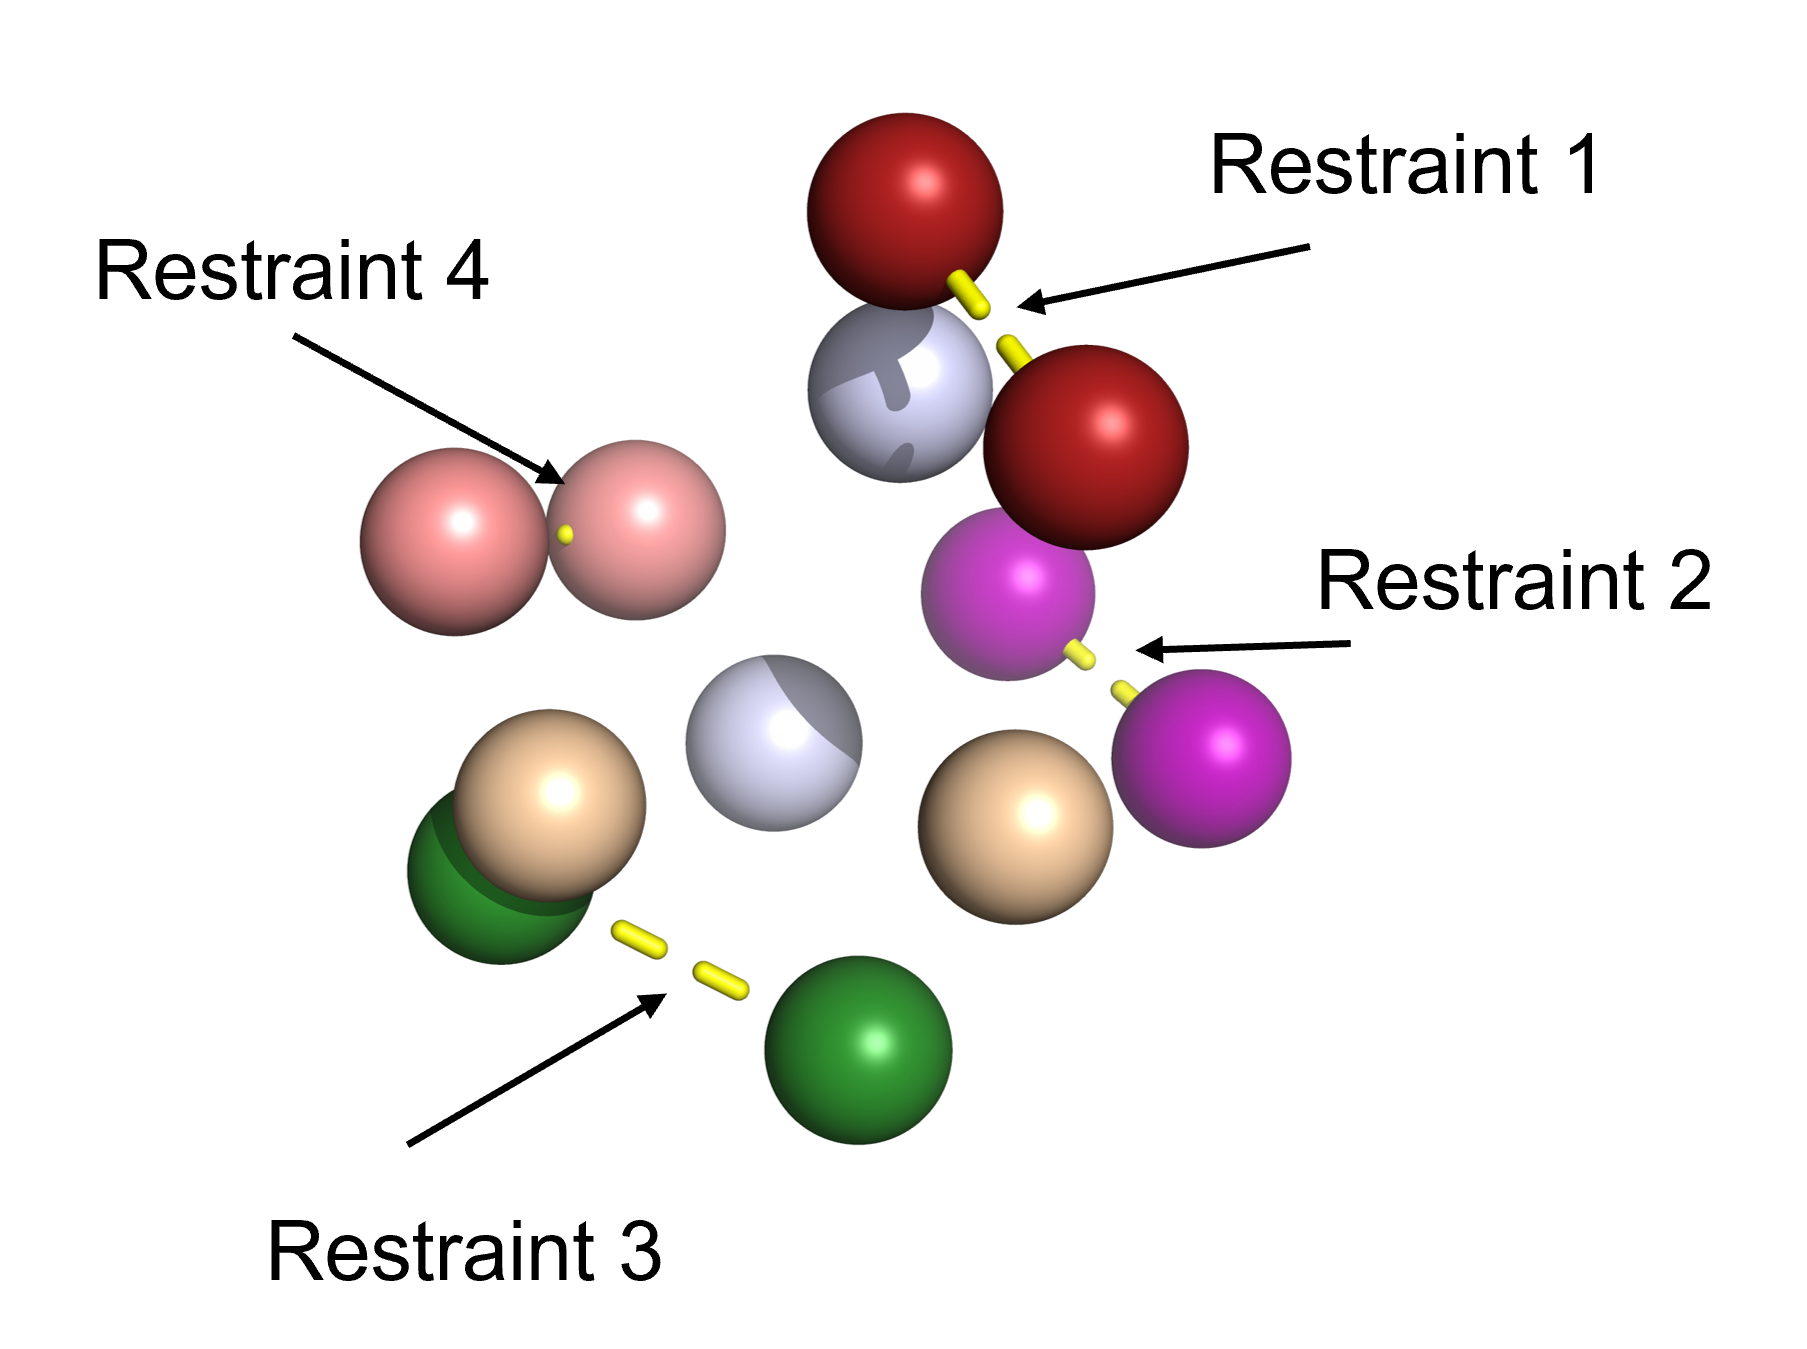
\includegraphics[width=\textwidth]{fig/results/algorithm/punktewolke_6_greedy_annotated.png}
        \caption{}
        \label{fig: greedyApproach_6Partikels}
    \end{subfigure}
    \begin{subfigure}{0.45\columnwidth}
        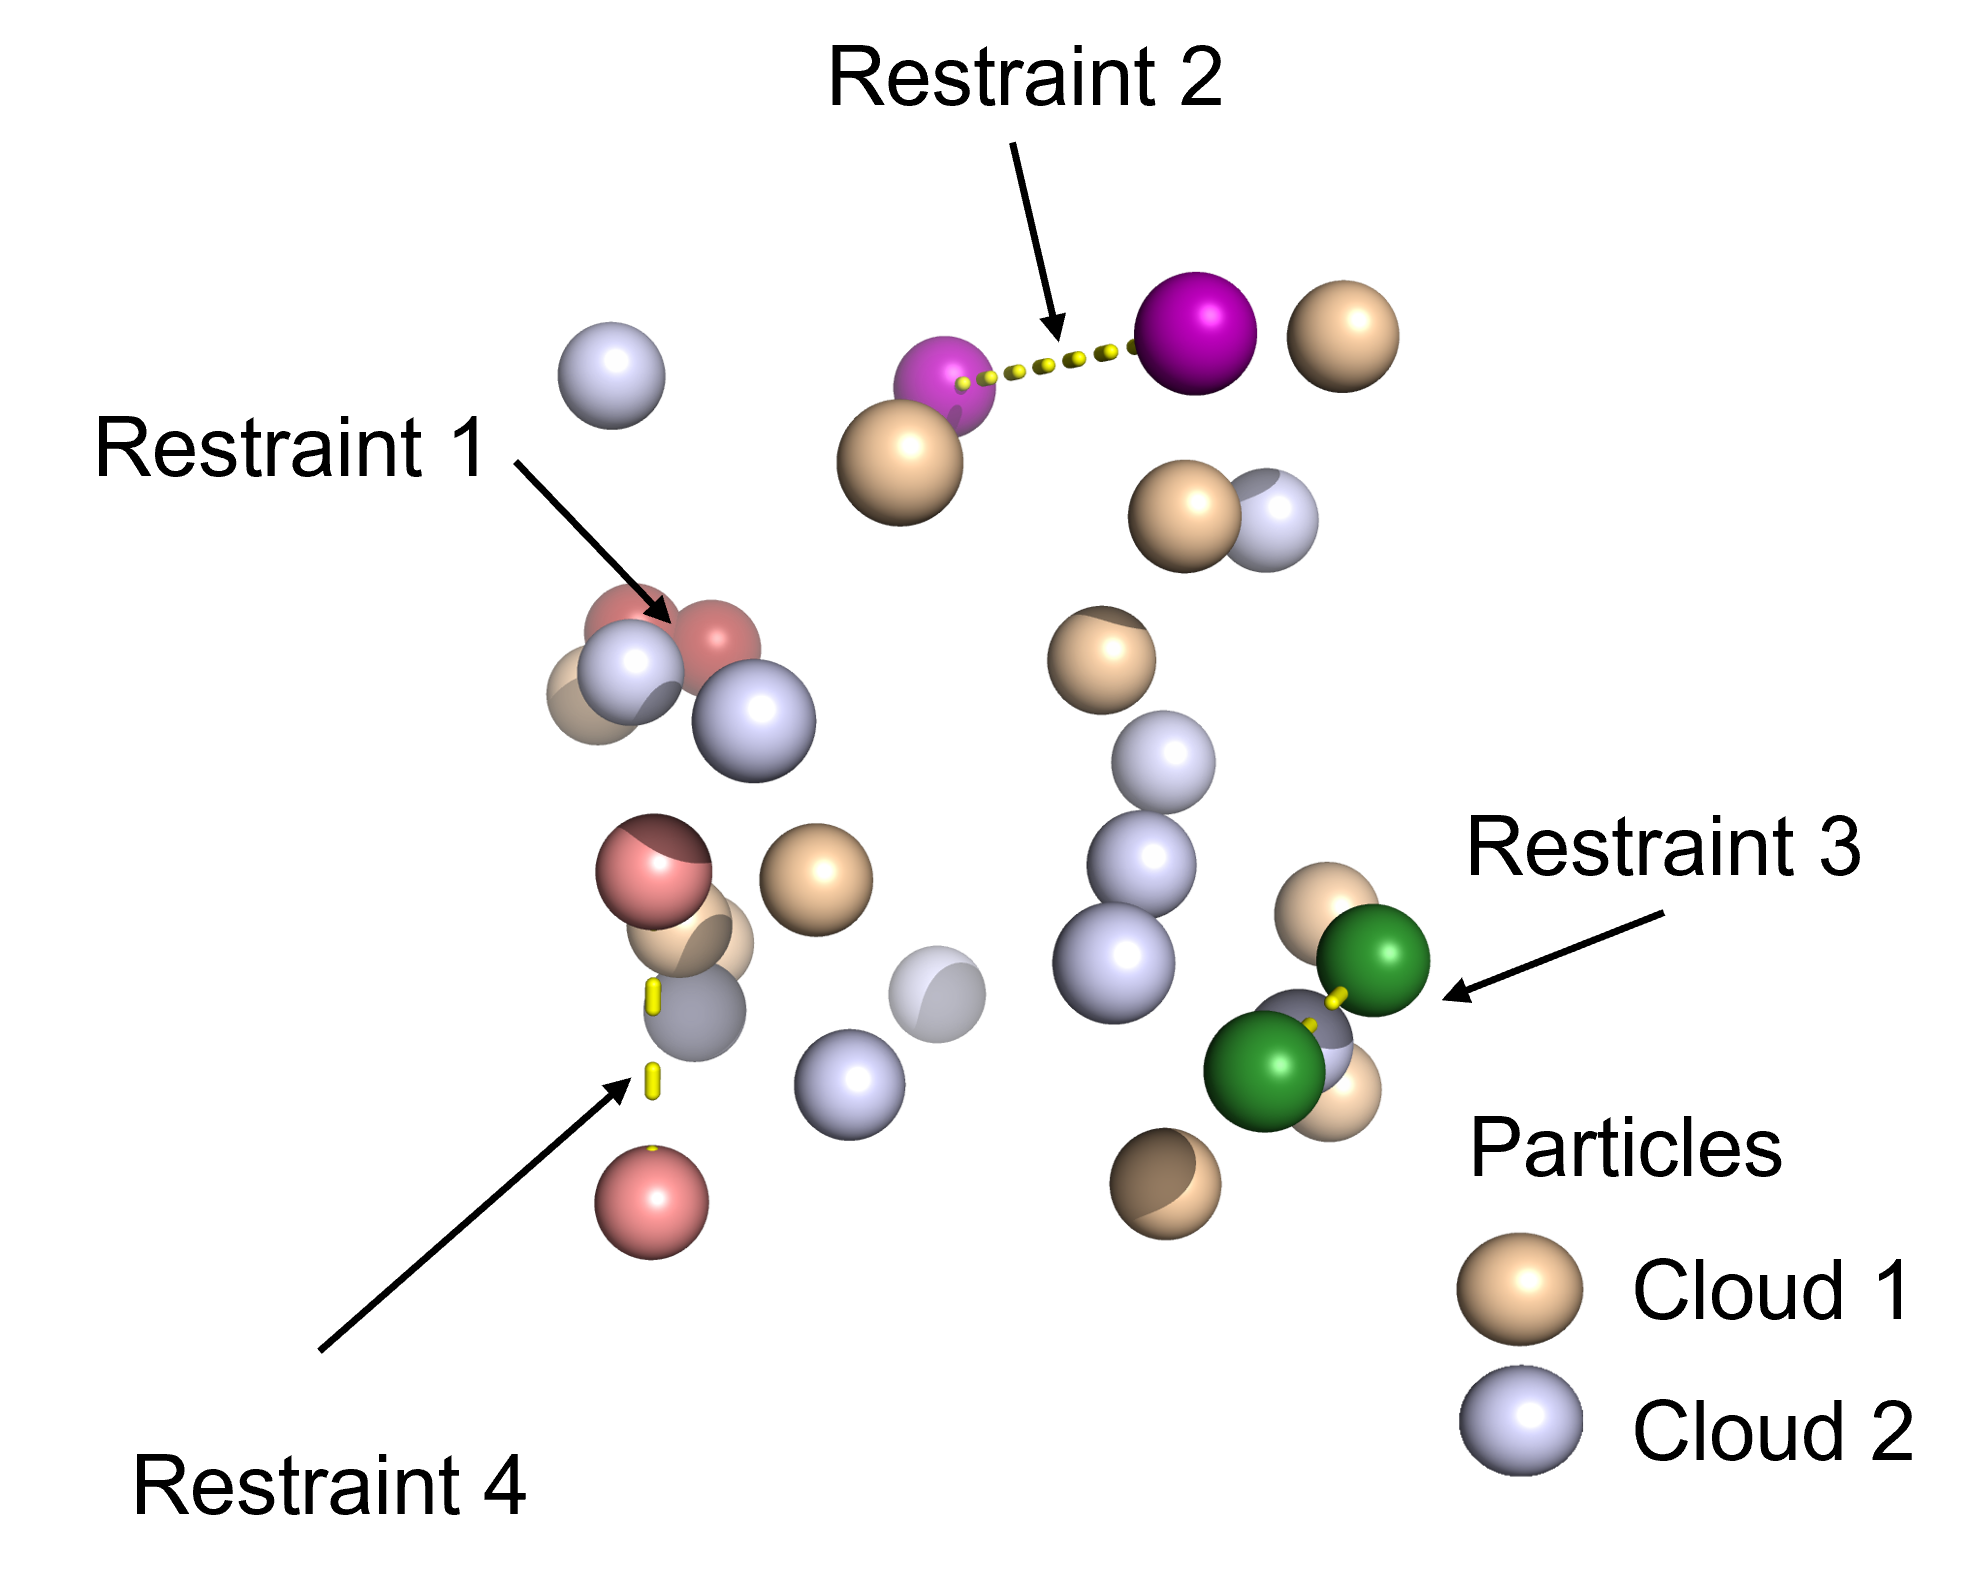
\includegraphics[width=\textwidth]{fig/results/algorithm/punktewolke_15_greedy_annotated.png}
        \caption{}
        \label{fig: greedyApproach_15Partikels}
    \end{subfigure}
    \caption{Comparison of algorithms to select distance restraints on toy systems. (a): Time complexity as a function of the number of particles in the system for the brute-force approaches BF-maxCHV (red) and BF-maxD (blue), and the greedy algorithm (yellow). (b): Distance metric as a function of the number of particles in the system for the brute-force approaches (red and blue), the greedy algorithm (yellow), and random selection with 100 trials (purple). (c): CHV as a function of the number of particles in the system. (d and e): Final distance restraints selected by the greedy algorithm for 12 (d) and 30 (e) particles. The restrained atoms are colored in green, red, pink and rose, and connected by yellow dashed lines. The two particle clouds are colored in wheat and light blue.}
    \label{fig: ToyModels}
\end{figure}

Comparison of the sum of all distances between restraint midpoints shows that BF-maxD (optimizing for the maximal distance between all midpoints of the selected restraints) yields the best results with the largest distances (blue line in Figure \ref{fig: ToyModels}b). The second brute-force algorithm BF-maxCHV (optimizing for the CHV defined by the restraint midpoints) and our greedy algorithm give comparable results to BF-maxD. All three approaches are very good at maximizing the distance between the selected restraints. Random selection with 100 trials (negative control), on the other hand, performs significantly worse.
Second, we compared the approaches based on the CHV generated by the selected restraints (Figure \ref{fig: ToyModels}c). Here, the BF-maxCHV approach yields the best results as expected, while BF-maxD and the greedy algorithm perform similar to each other. The difference in CHV between the latter two approaches and BF-maxCHV increases with increasing number of particles in the toy system. This may be due to the growing number of possible choices, or due to the fact that the distance metric used in BF-maxD and the greedy algorithms is suboptimal. All approaches clearly outperform random selection.
%
The greedy algorithm in RestraintMaker can thus be seen as a trade-off between optimizing a metric (distance or CHV) and limiting the required computing time. It is the fastest algorithm among the ones tested and yields comparable results to the brute-force approaches. 

\subsection{Pairwise Calculation of Relative Hydration Free Energies}
To assess the quality of the selected distance restraints, the greedy algorithm in RestraintMaker was tested with a set of 16 small molecules with experimentally available hydration free energies. First, the relative hydration free energies were calculated between molecule \textbf{12} and the 15 other molecules using TI (Figure \ref{fig: Pairwise_TI_M030_Graph}). 

\subsubsection{Free Energy Calculation}
The resulting $\Delta \Delta G_\text{hyd}^\text{TI,indirect}$ agree very well with the experimental values,\cite{Wolfenden1987,Rizzo2006,Nicholls2008,Guthrie2009,Guthrie2014,Mobley2014} with a root-mean-square error (RMSE) of $4.1$~kJ/mol, a mean absolute error (MAE) of $3.1$~kJ/mol (Figure \ref{fig: pairCorr}, left) and a Spearman correlation coefficient $r_{\text{Spearman}}$ of 0.87.
The numerical values are reported in Table \ref{SITab: FE_M030_Graph},
and the corresponding $\langle \partial V(\lambda)/\partial\lambda \rangle$ curves in water and vacuum in Figures \ref{SIfig:TI_vacuum_curve} and  \ref{SIfig:TI_water_curve}. 

\begin{table}[H]
\caption{$\Delta \Delta G_\text{hyd}$ for the 16 small molecules from experiment, the absolute free-energy calculations with TI taken from the ATB server\cite{Stroet2018} (TI, abs), and the pairwise relative free-energy calculations with TI and linked dual topology (TI, rel).
The uncertainty estimate was calculated via Gaussian error propagation of the provided errors. The experimental uncertainty for molecule 11 was set to a default value of 2.5~kJ/mol\cite{Mobley2014}, as the uncertainty was not reported in the original source\cite{Wolfenden1987}. The RMSE and its uncertainty were estimated with a 100 fold bootstrap approach. The accumulated simulation time is split into preparation (pre-processing, equilibration) and production run. The data is displayed graphically in Main Article Figure 9}
\begin{center}
\begin{adjustbox}{max width=\textwidth}
\begin{tabular}{ | c c |c |c|c|}
\hline
  \multicolumn{2}{|c|}{Ligands} & \multicolumn{1}{c|}{Experiment} &\multicolumn{1}{c|}{$\Delta\Delta G_\text{hyd}^\text{TI,direct}$}&\multicolumn{1}{c|}{$\Delta\Delta G_\text{hyd}^\text{TI,indirect}$}\\ 
    $i$ & $j$ & [kJ/mol] & [kJ/mol] & [kJ/mol]  \\
  \hline \hline
        1 &  12 &  $18.5 ~\pm~ 2.5$ ~\cite{Guthrie2014,Rizzo2006}&  $26.2 ~\pm~ 0.8$ &  $  17.5 ~\pm~ 0.7$\\
        2 &  12 &  $11.9 ~\pm~ 2.7$  ~\cite{Guthrie2014,Rizzo2006}  &  $14.4 ~\pm~ 0.7$ &  $  8.6 ~\pm~ 0.6 $\\
        3 &  12 &  $14.8 ~\pm~ 3.1$  ~\cite{Guthrie2014,Rizzo2006}  &  $22.4 ~\pm~ 0.7$ &  $ 15.2 ~\pm~ 0.9 $\\
        4 &  12 &  $15.9 ~\pm~ 3.5$  ~\cite{Rizzo2006} &  $15.3 ~\pm~ 0.6$ &  $  9.4 ~\pm~ 0.4 $\\
        5 &  12 &   $36.1 ~\pm~ 2.8$  ~\cite{Guthrie2014,Rizzo2006}  &  $48.2 ~\pm~ 0.4$ &  $ 46.9 ~\pm~ 0.8 $\\
        6 &  12 &   $28.1 ~\pm~ 3.5$  ~\cite{Rizzo2006}  &  $36.1 ~\pm~ 0.6$ & $  30.5 ~\pm~ 0.5 $\\
        7 &  12 &   $10.6 ~\pm~ 2.5$  ~\cite{Guthrie2009,Rizzo2006} &  $22.8 ~\pm~ 0.5$ &  $  9.5 ~\pm~ 0.9 $\\
        8 &  12 &   $ 1.6 ~\pm~ 3.5$  ~\cite{Mobley2014,Rizzo2006} &  $ 5.2 ~\pm~ 0.7$ &  $ 3.0 ~\pm~ 1.2 $\\
        9 &  12 &   $27.5 ~\pm~ 3.5$  ~\cite{Rizzo2006}  &  $30.2 ~\pm~ 0.6$ &  $ 25.7 ~\pm~ 0.5 $\\
        10 &  12 &   $ 8.0 ~\pm~ 3.5$  ~\cite{Rizzo2006}  &  $ 6.5 ~\pm~ 0.6$ &  $  5.9 ~\pm~ 0.5 $\\
        11 &  12 &   $20.4  ~\pm~ 3.5$  ~\cite{Wolfenden1987,Rizzo2006}&  $17.0 ~\pm~ 0.6$ &  $ 14.8 ~\pm~ 0.39 $\\
        12 &  13 &   $16.8 ~\pm~ 3.5$  ~\cite{Rizzo2006} &  $18.6 ~\pm~ 0.6$ &  $ 16.6 ~\pm~ 0.5 $\\
        12 &  14 &   $15.9 ~\pm~ 3.5$  ~\cite{Rizzo2006}&  $24.9 ~\pm~ 0.6$ &  $ 20.5 ~\pm~ 0.5 $\\
        12 &  15 &    $6.2 ~\pm~ 2.6$  ~\cite{Rizzo2006, Nicholls2008}  &  $14.9 ~\pm~ 0.7$ &  $ 10.3 ~\pm~ 0.4 $\\
        12 &  16 &   $25.5 ~\pm~ 3.5$  ~\cite{Rizzo2006} &  $26.1 ~\pm~ 0.6$ &   $ 24.0 ~\pm~ 0.4 $\\
  \hline
        \multicolumn{2}{|c|}{RMSE} &          & $6.7 ~\pm~ 0.3$ & $4.1 ~\pm~ 0.3 $\\
        \multicolumn{2}{|c|}{MAE} &           & $5.5 ~\pm~ 3.9$ & $3.1 ~\pm~ 2.7$ \\
        %\multicolumn{2}{c|}{$r_{\text{Pearson}}$} & & 0.90  & 0.93 \\
        \multicolumn{2}{|c|}{$r_{\text{Spearman}}$} &  & $0.84$ & $0.87$  \\
        \multicolumn{2}{|c|}{$t_{preparation}$} & & &  $630$~ns \\
        \multicolumn{2}{|c|}{$t_{production}$} & &$112 - 272~ns$ &  $3150$~ns \\
        \hline
\end{tabular}
\end{adjustbox}
\end{center}
\label{SITab: FE_M030_Graph}
\end{table}


\begin{figure}[H]
    \centering
    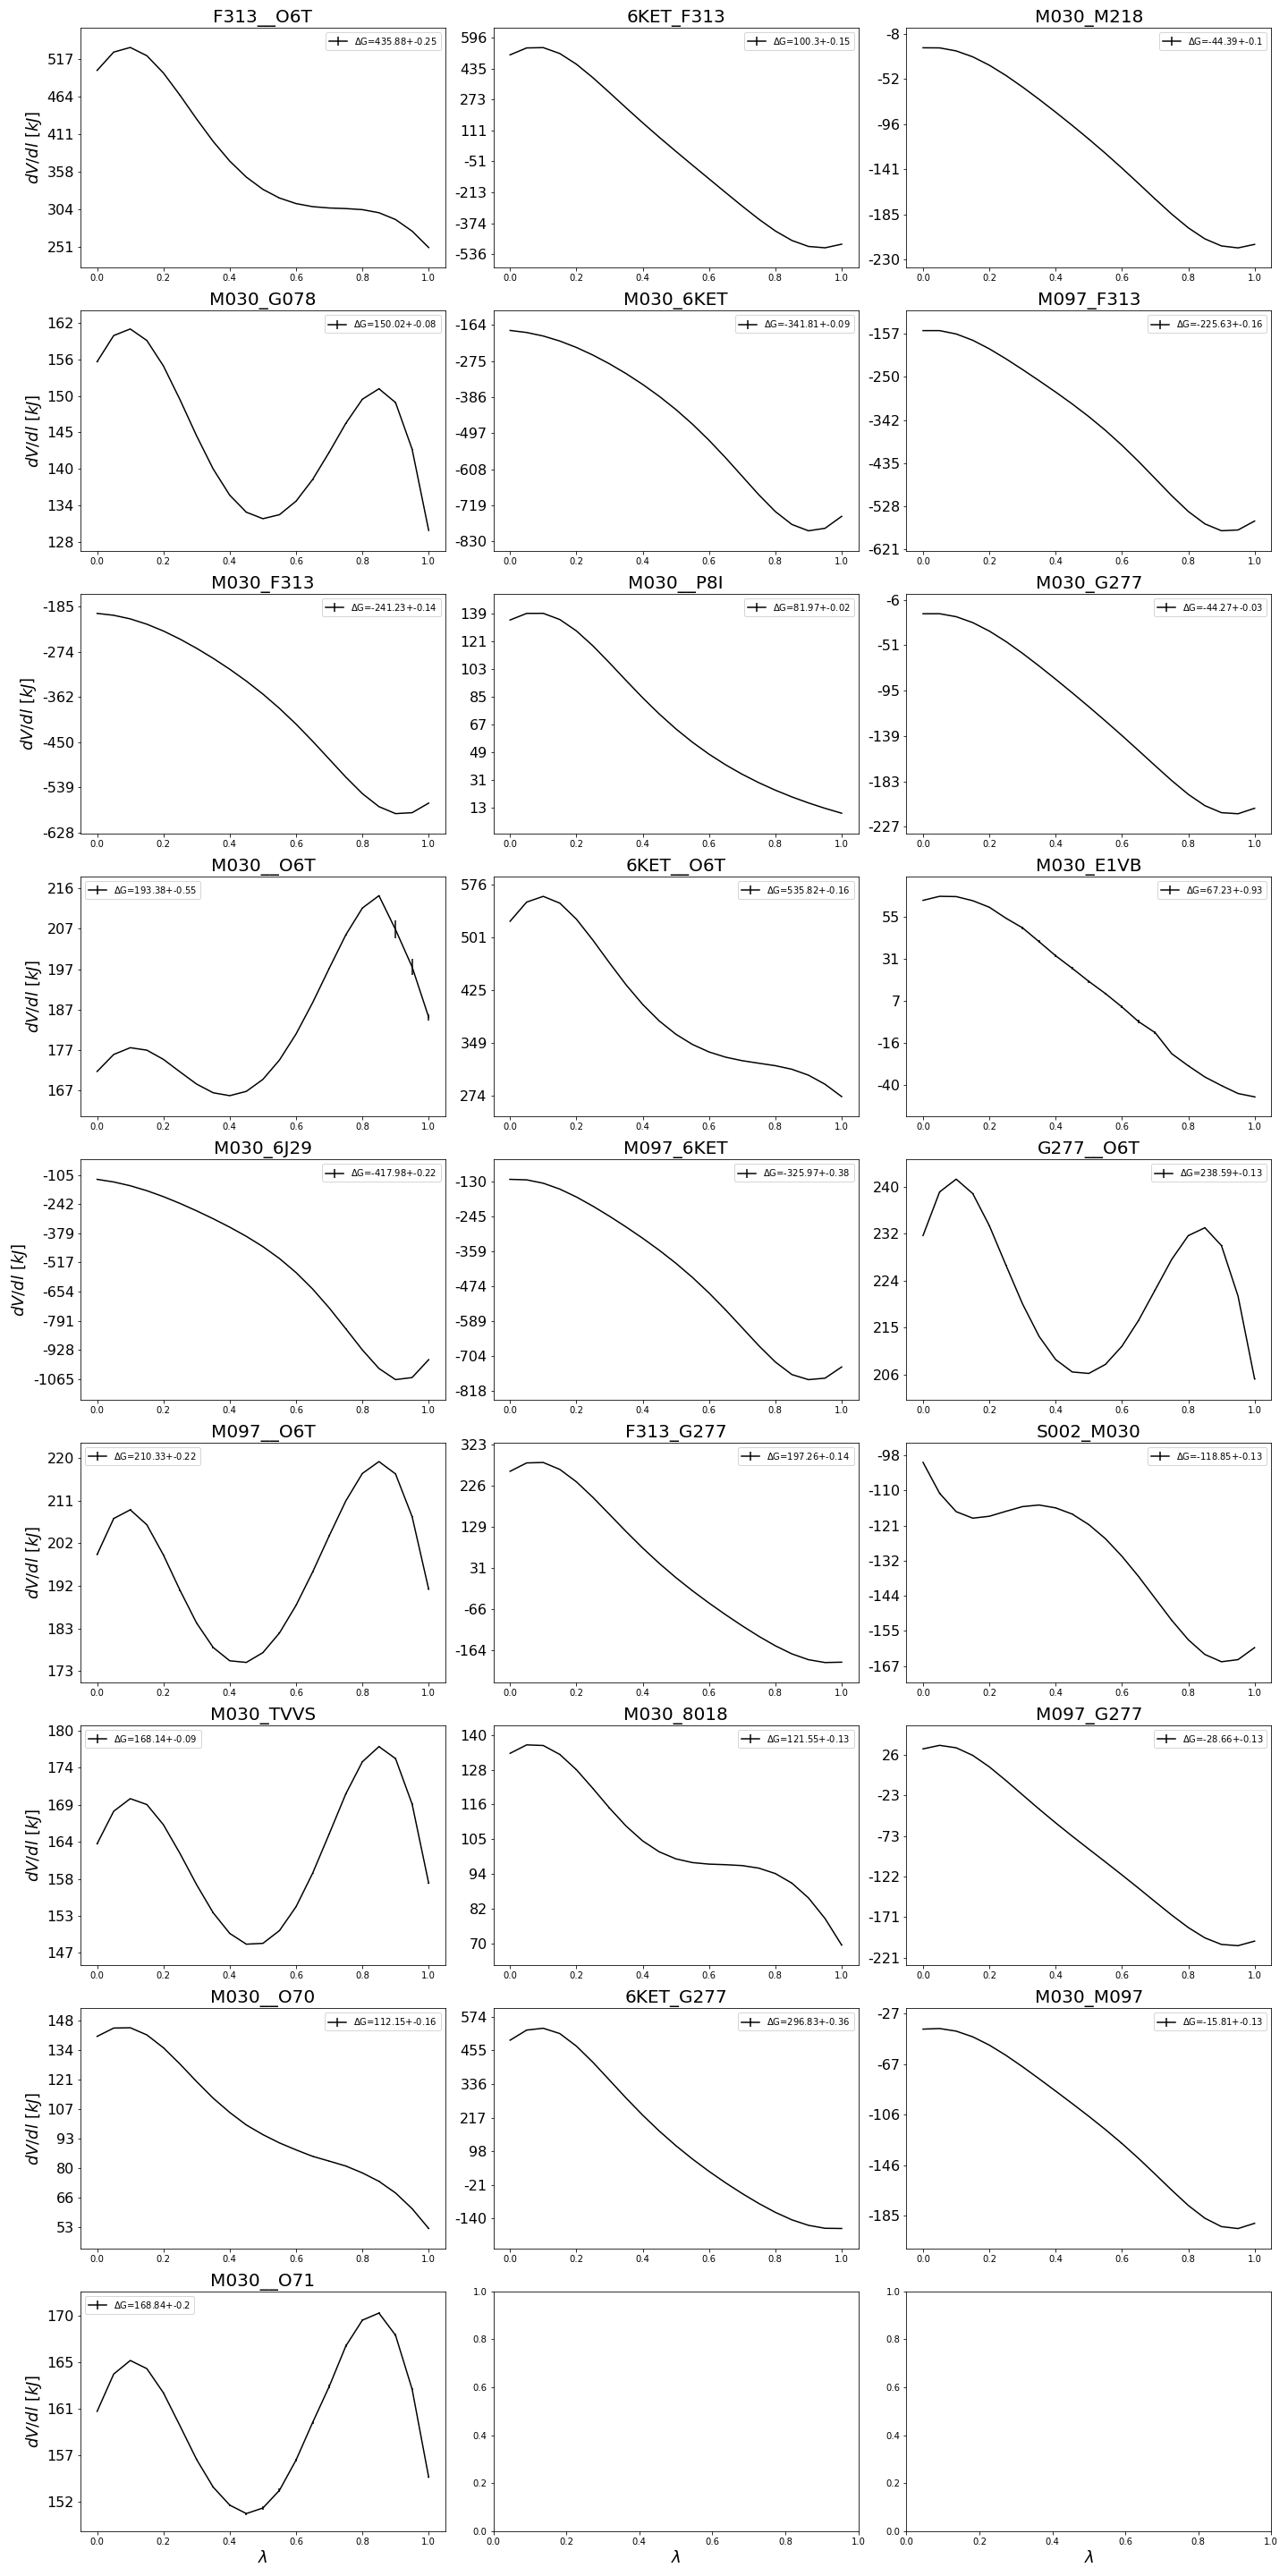
\includegraphics[width=0.8\textwidth]{fig/SI/dG_convergence/TI_vacuum_lambda_curves.png}
    \caption{$\left< \frac{\partial V(\lambda)}{\partial \lambda} \right>_{\lambda}$ as a function of $\lambda$ for the 15 pairwise TI calculations in vacuum. The production run was 5~ns per $\lambda$-point.}
    \label{SIfig:TI_vacuum_curve}
    \end{figure}

\begin{figure}[H]
    \centering
    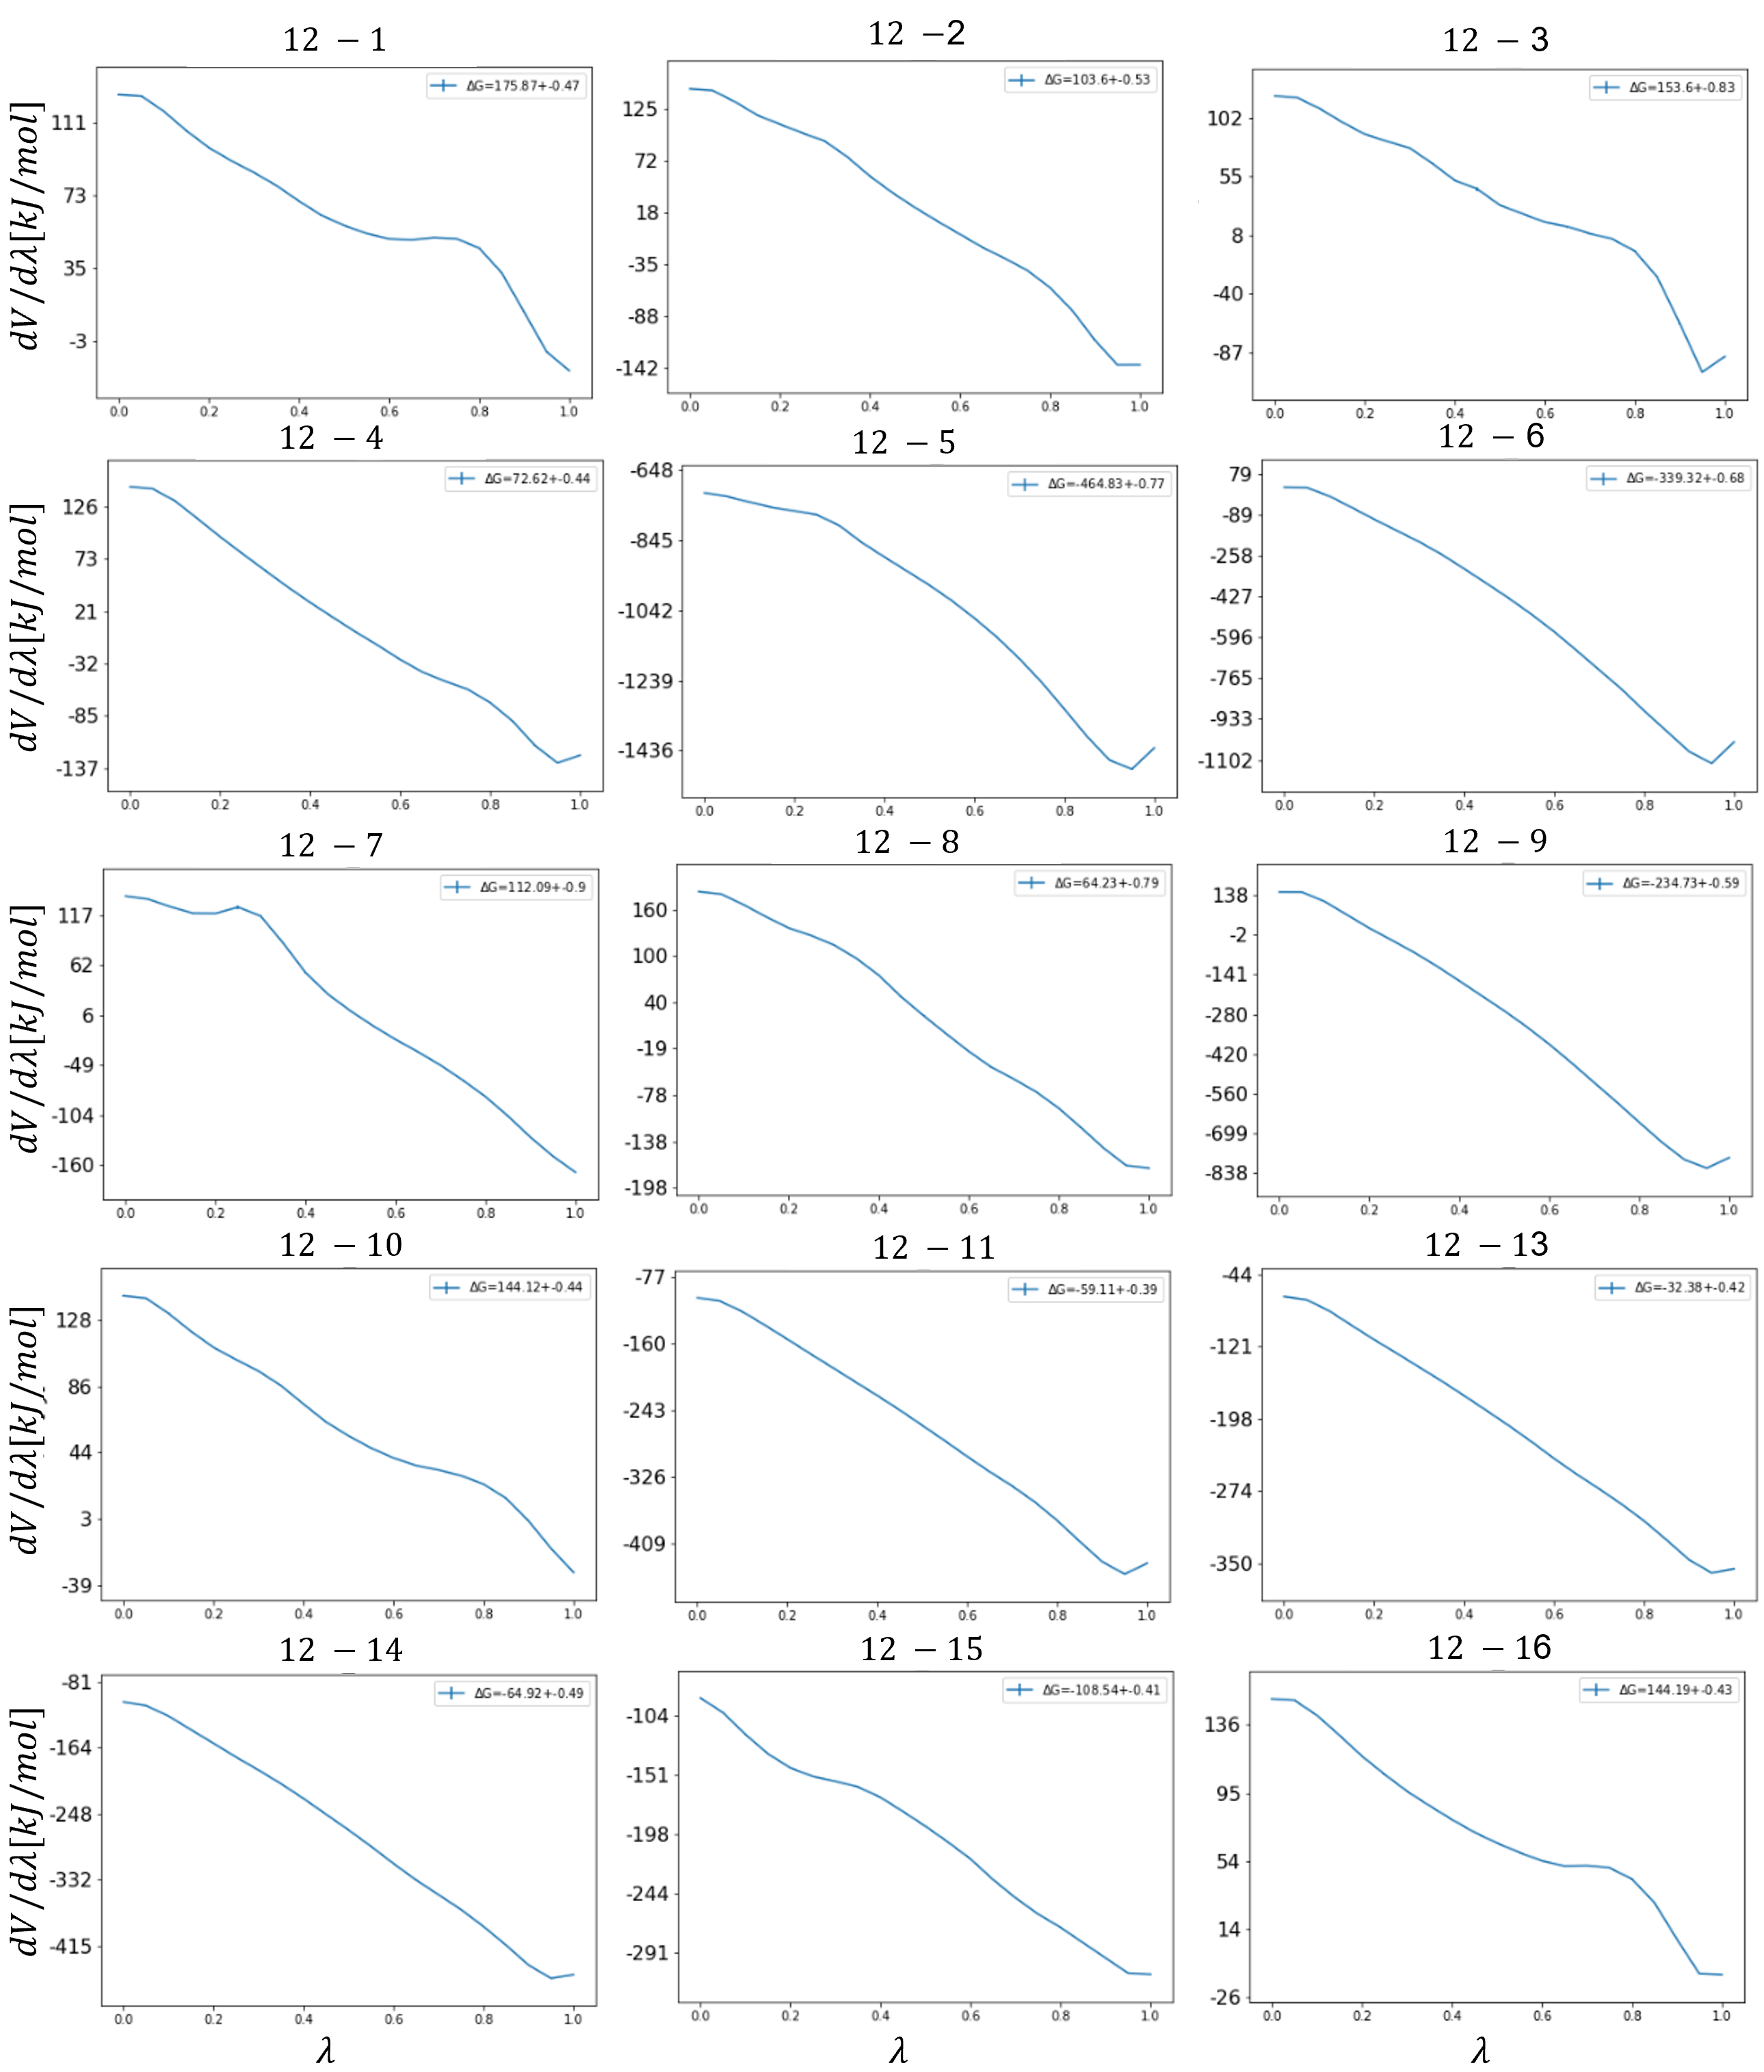
\includegraphics[width=0.8\textwidth]{fig/SI/dG_convergence/TI_water_lambda_curves.png}
    \caption{$\left< \frac{\partial V(\lambda)}{\partial \lambda} \right>_{\lambda}$ as a function of $\lambda$ for the 15 pairwise TI calculations in water. The production run was 5~ns per $\lambda$-point.}
    \label{SIfig:TI_water_curve}
\end{figure}

%----------------------------
\FloatBarrier
For comparison, $\Delta \Delta G_{hyd}^\text{TI,direct}$ values were derived from the calculated absolute hydration free energies reported on the ATB server,\cite{Stroet2018} which were carried out with TI using the same topologies. The $\Delta \Delta G_{hyd}^{TI,direct}$ values deviate a bit more from experiment with an RMSE of $6.7$~kJ/mol, a MAE of $5.5$~kJ/mol and a $r_{\text{Spearman}}$ of 0.84 (Figure \ref{fig: pairCorr}, center).
Generally, the results of the direct\cite{Stroet2018} and indirect TI calculations agree well with each other (Figure \ref{fig: pairCorr}, right). Note that for the molecule pair \textbf{5} - \textbf{12}, a similarly large deviation from experiment is observed in both types of TI calculations ($10.7$~kJ/mol and $12.1$~kJ/mol, respectively), suggesting either a force-field deficiency or a problematic experimental value.

\begin{figure}[h!]
    \centering
    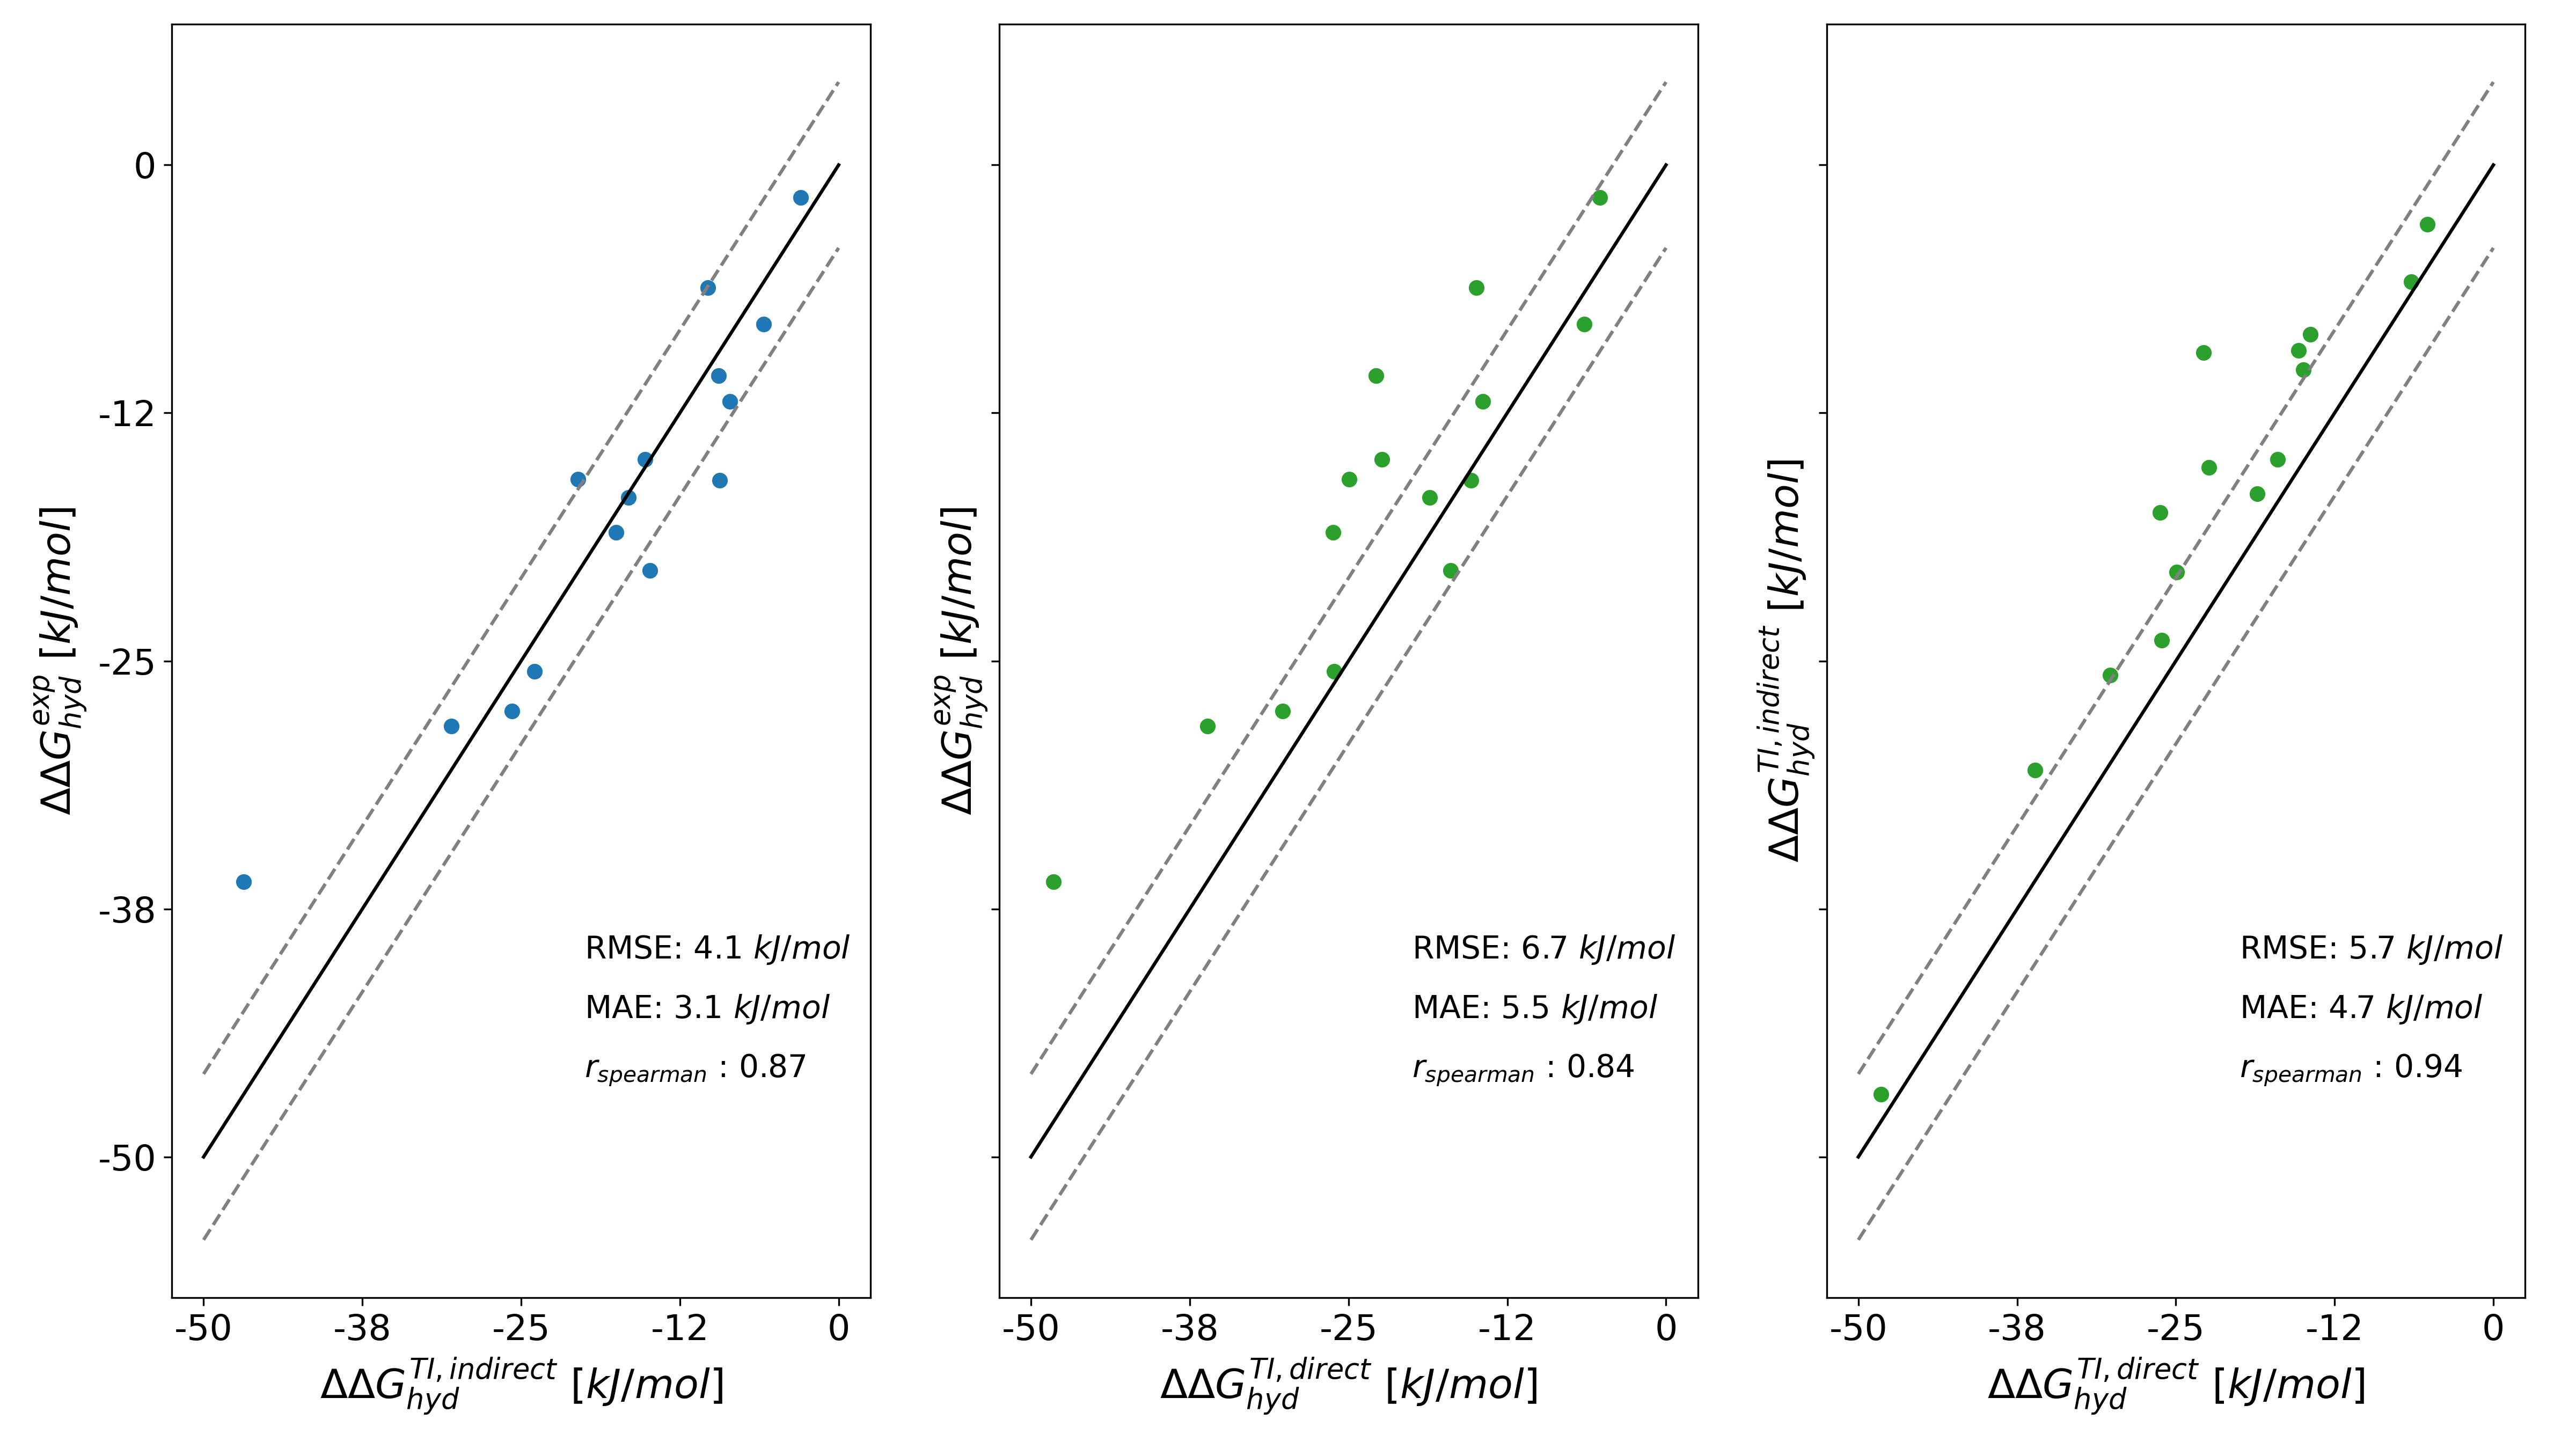
\includegraphics[width=\textwidth]{fig/results/pairwise/FE/M030_graph_ddG_solv_correlation_ATB_TI.png}
    \caption{Comparison of the relative hydration free energies $\Delta \Delta G_{hyd}$ (with molecule \textbf{12} as reference) for the 16 small molecules between experiment (exp), the pairwise relative free-energy calculations with TI and linked dual topology (TI, indirect), and the absolute free-energy calculations with TI taken from the ATB server\cite{Stroet2018} (TI, direct). The numerical values are given in Table \ref{SITab: FE_M030_Graph}} 
    \label{fig: pairCorr}
\end{figure}


\begin{figure}[H]
    \centering
    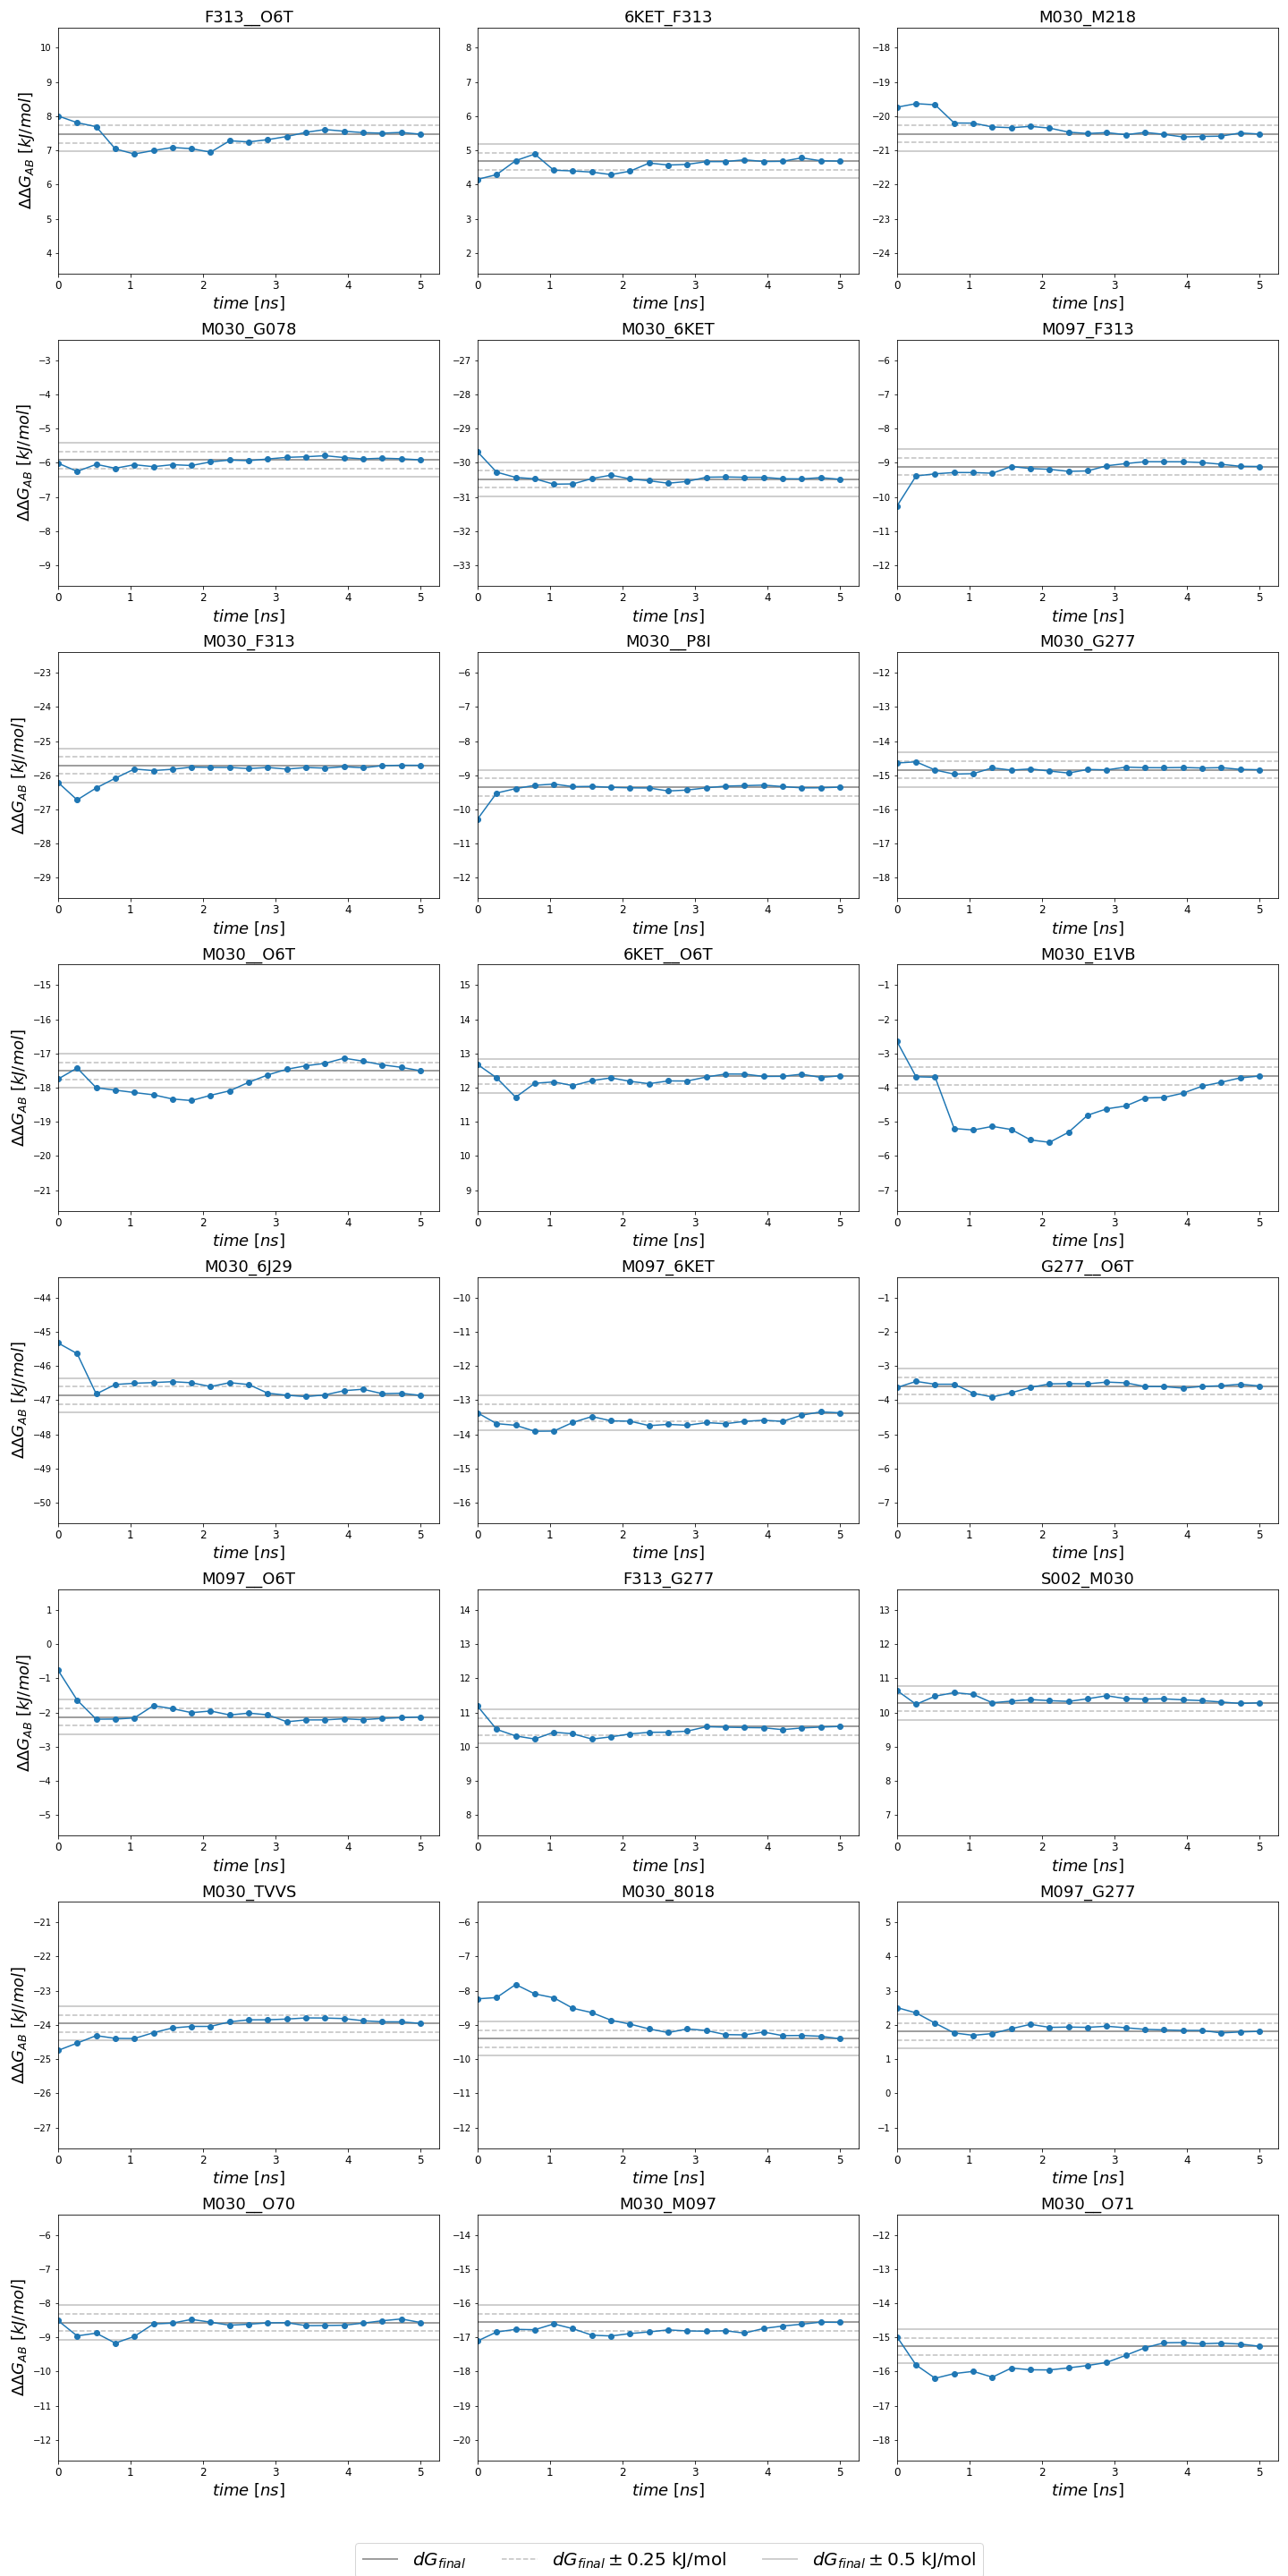
\includegraphics[width=0.8\textwidth]{fig/SI/dG_convergence/ddG_TI_convergence.png}
    \caption{Convergence of $\Delta \Delta G_\text{hyd}$ as a function of the simulation time per $\lambda$-point for the 15 pairwise TI calculations.}
    \label{fig: SI_figure df_convergence_TI}
\end{figure}


\subsubsection{Sampling}
%Coordinate analysis - Translation
It is crucial for the linked dual topology approach that the applied distance restraints do not distort the conformational sampling of the molecules. 
For this, the relative translational motion of the two aligned molecules was analyzed for each $\lambda$-window and molecule pair by calculating the fluctuation of the distance between the COGs of the restrained atoms in the central rings of the two molecules. Figure \ref{fig: pairCOGDist_TIStarMa} shows both the standard deviation and the maximum observed distance between the two COGs. 

\begin{figure}[h!]
    \centering
    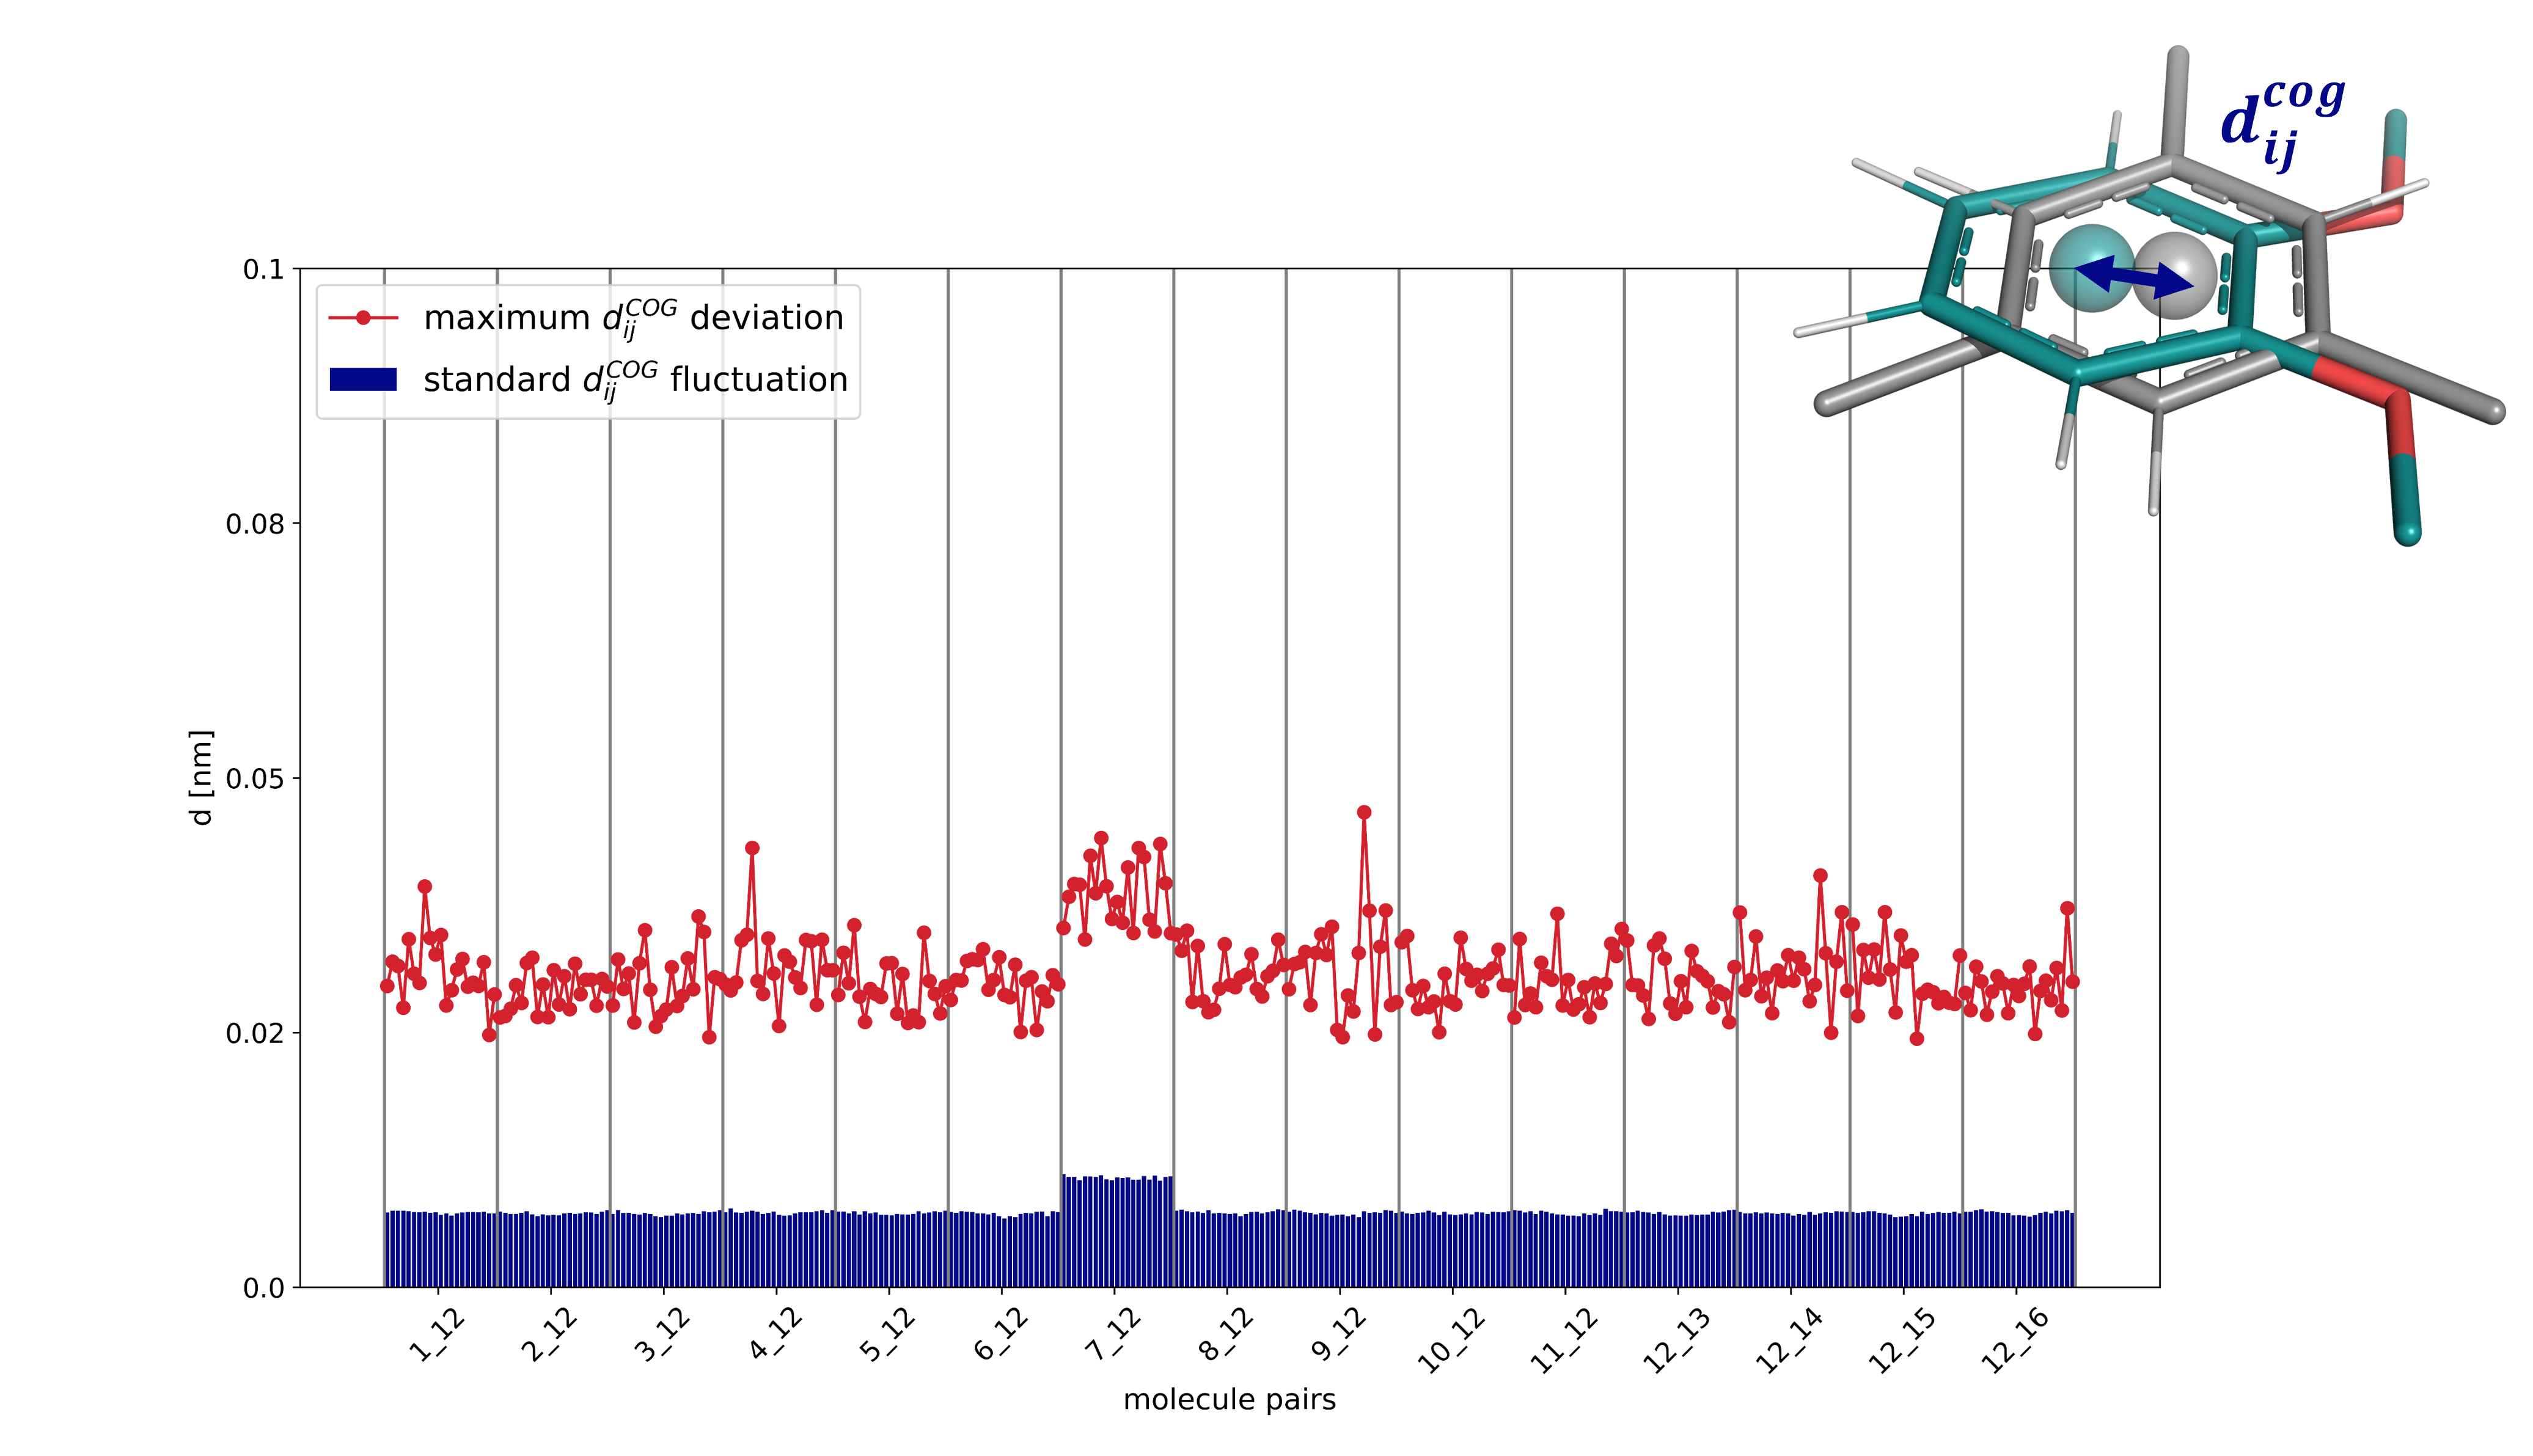
\includegraphics[width=\textwidth]{fig/results/pairwise/sampling/TI_pairwise_dCOG_fluctuations.png}
    \caption{Standard deviation of the distance distribution (blue) and maximum distance (red) between the COGs of the central rings of the molecule pairs in the TI simulations in water. The COG was calculated for the restrained atoms in the rings. The horizontal axis shows for each molecule pair the different $\lambda$-windows between 0 and 1.}
    \label{fig: pairCOGDist_TIStarMa}
\end{figure}


The standard deviation is close to zero for all pairs, indicating that the two cores overlap well given the chosen restraints. Maximum distances are around $0.03~$nm. For the pair \textbf{7} - \textbf{12}, the distances are slightly higher, which results from the fact that molecule \textbf{7} is a bridged bicycle. The force constant of $5000$~kJ$/($mol$\cdot$nm$^2)$ for the distance restraints was found to be a good compromise to ensure a tight overlap of the molecules without significantly perturbing their conformations. Note that the range of reasonable force constants is rather large and only for extremely high values (i.e. 50'000~kJ$/($mol$\cdot$nm$^2)$ or larger), does the restraining affect the free-energy results.

\begin{figure}[h!]
    \centering
    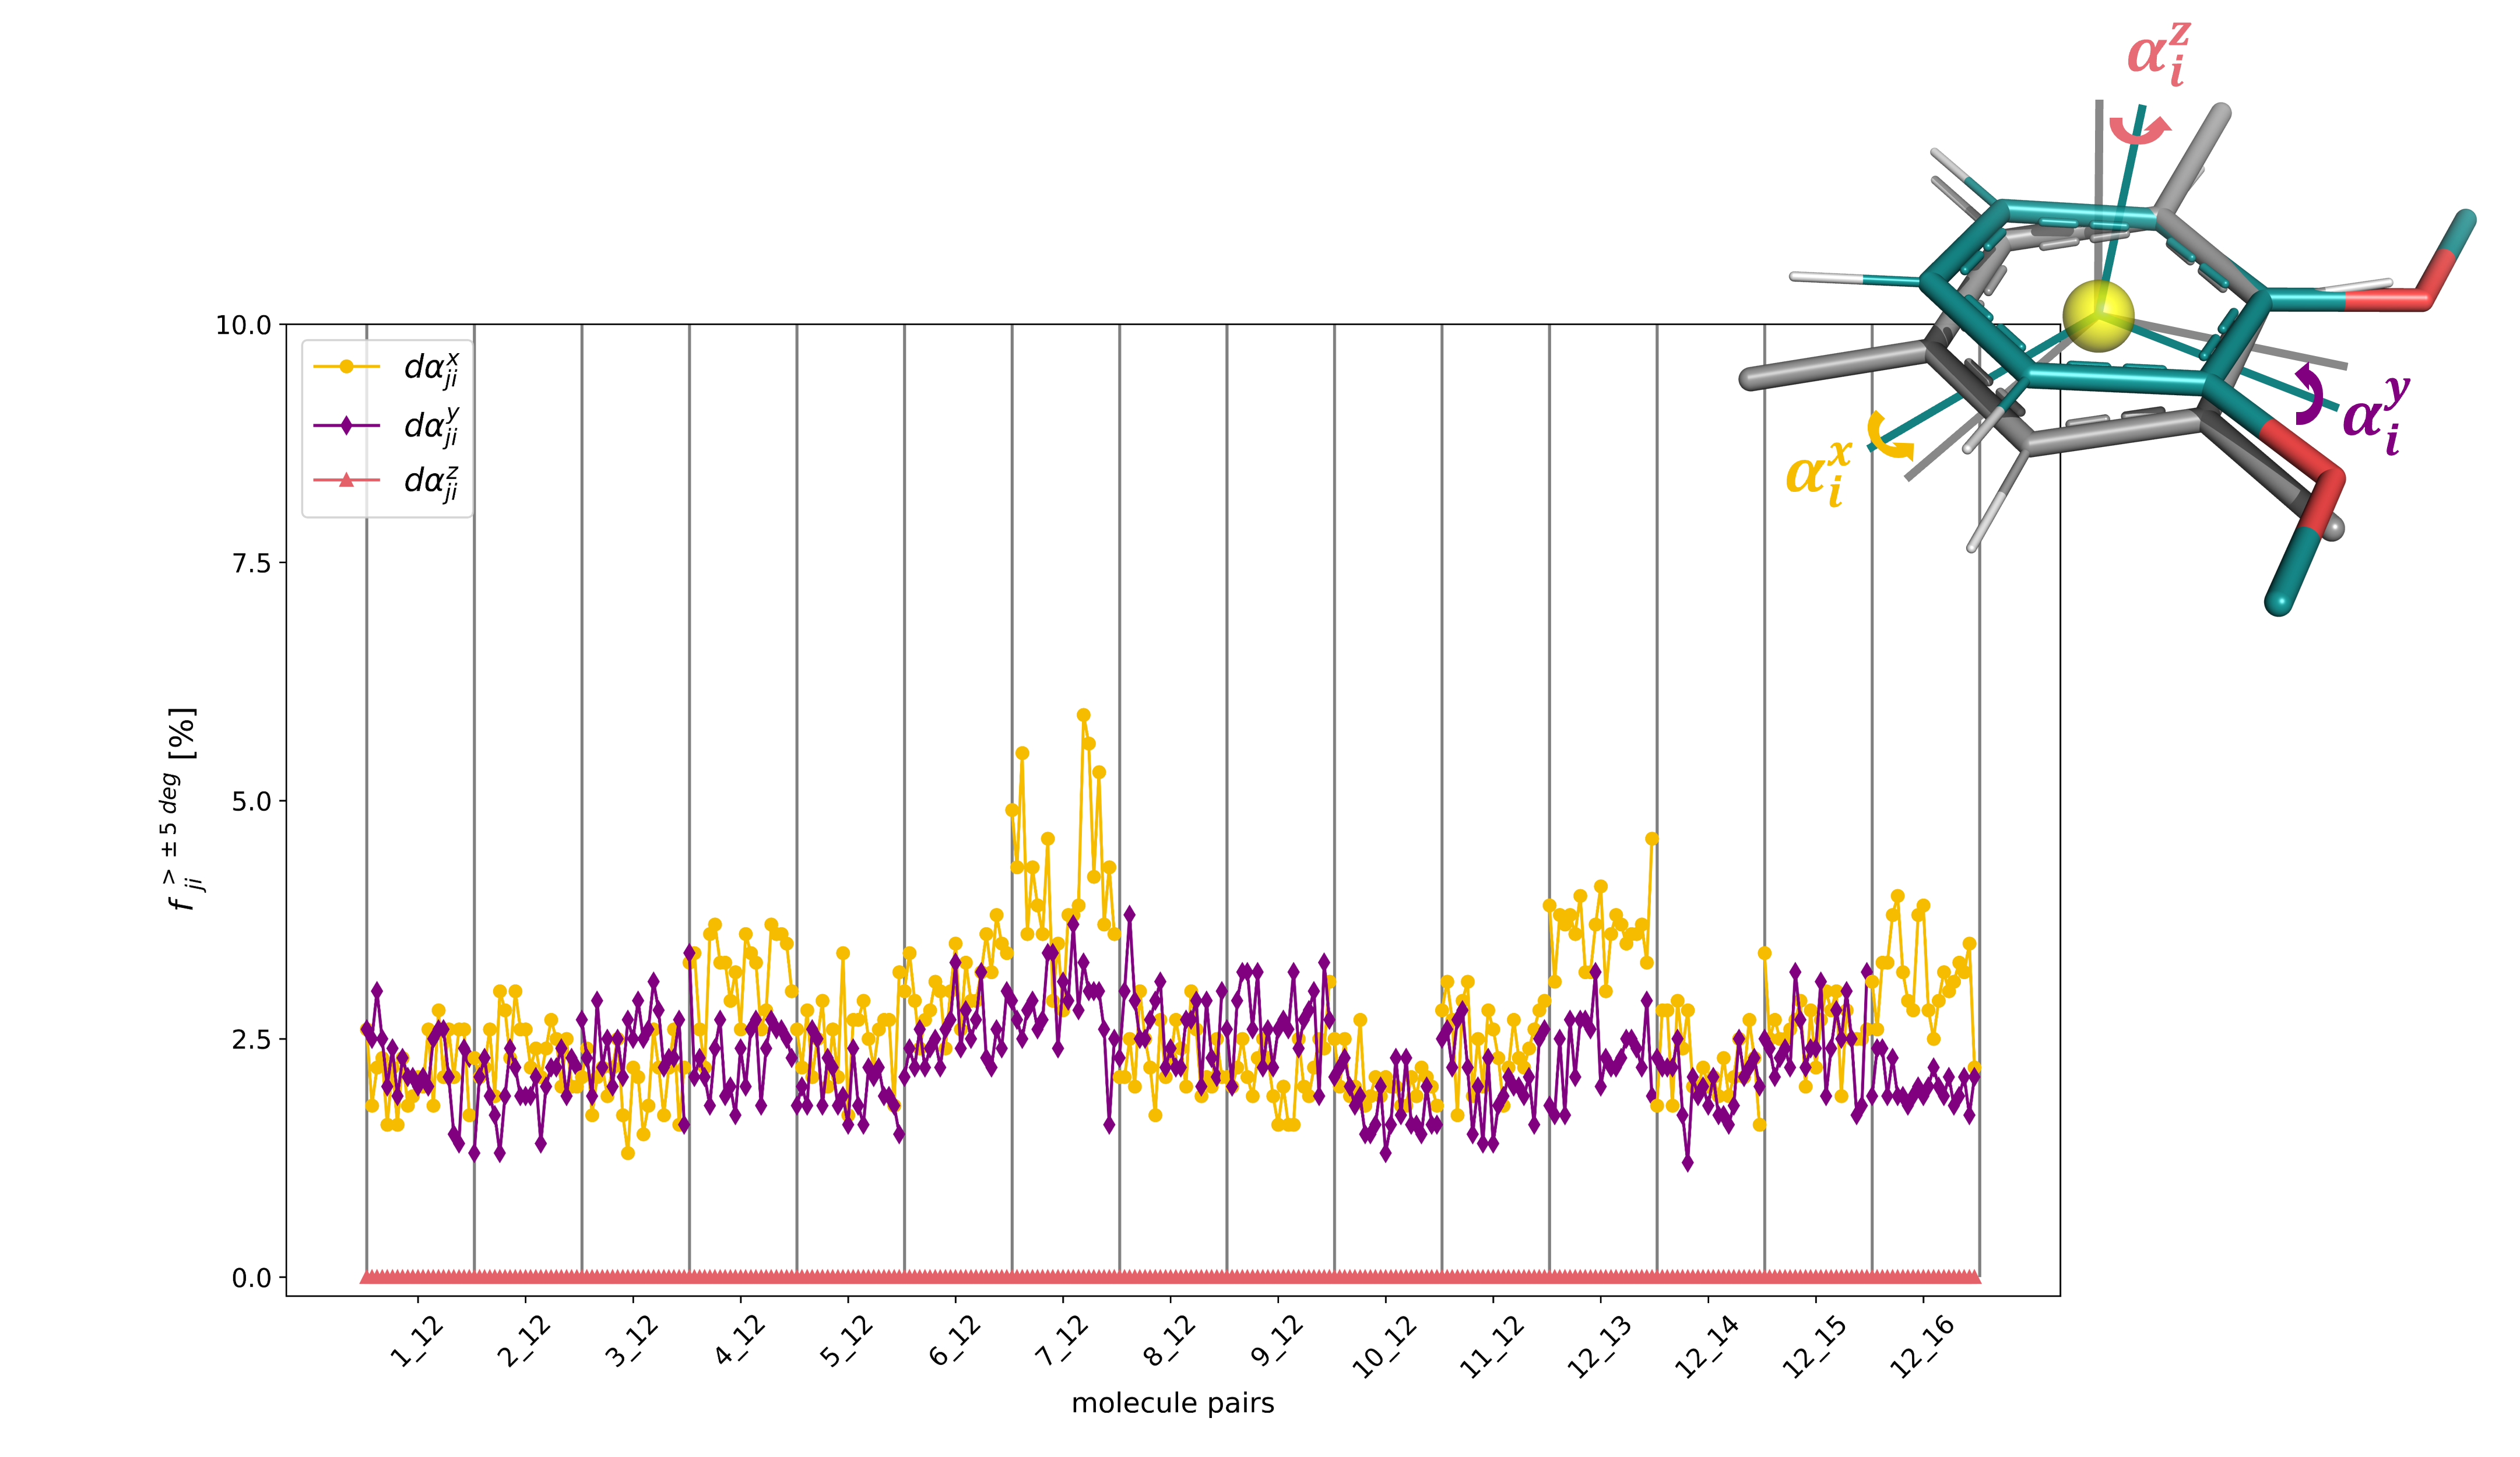
\includegraphics[width=\textwidth]{fig/results/pairwise/sampling/TI_pairwise_molecule_rotation.png}
    \caption{Fraction $f$ of frames in the TI simulations in water, in which the relative rotation around the $x$-axis (yellow), $y$-axis (purple), and $z$-axis (red) of the central rings of the molecule pair exceeds $5^{\circ}$. The horizontal axis shows for each molecule pair the different $\lambda$-windows between 0 and 1.}
    \label{fig: pairMolRotation_TIStarMap}
\end{figure}

%Coordinate analysis - Rotation
A similar analysis was carried out for the relative rotational motions of the molecules, considering the restrained atoms in the molecule pairs (Figure \ref{fig: pairMolRotation_TIStarMap}). In terms of the three Euler angles, a maximum relative rotation of $6.3^\circ$ was observed, which is reasonably small for one dimension. The largest fluctuation was again observed for the pair \textbf{7} - \textbf{12}. The rotation around the $z$-axis shows significantly smaller deviations compared to the other dimensions, because the two molecules need to rotate against each other in plane. In contrast, the rotations around the $x$ and $y$-axis correspond to a relative tilt of the molecules, which is easier to realize. 
 
 %-----------------------------------------
 \FloatBarrier
 
\begin{figure}[h!]
    \centering
    \begin{subfigure}{0.85\columnwidth}
        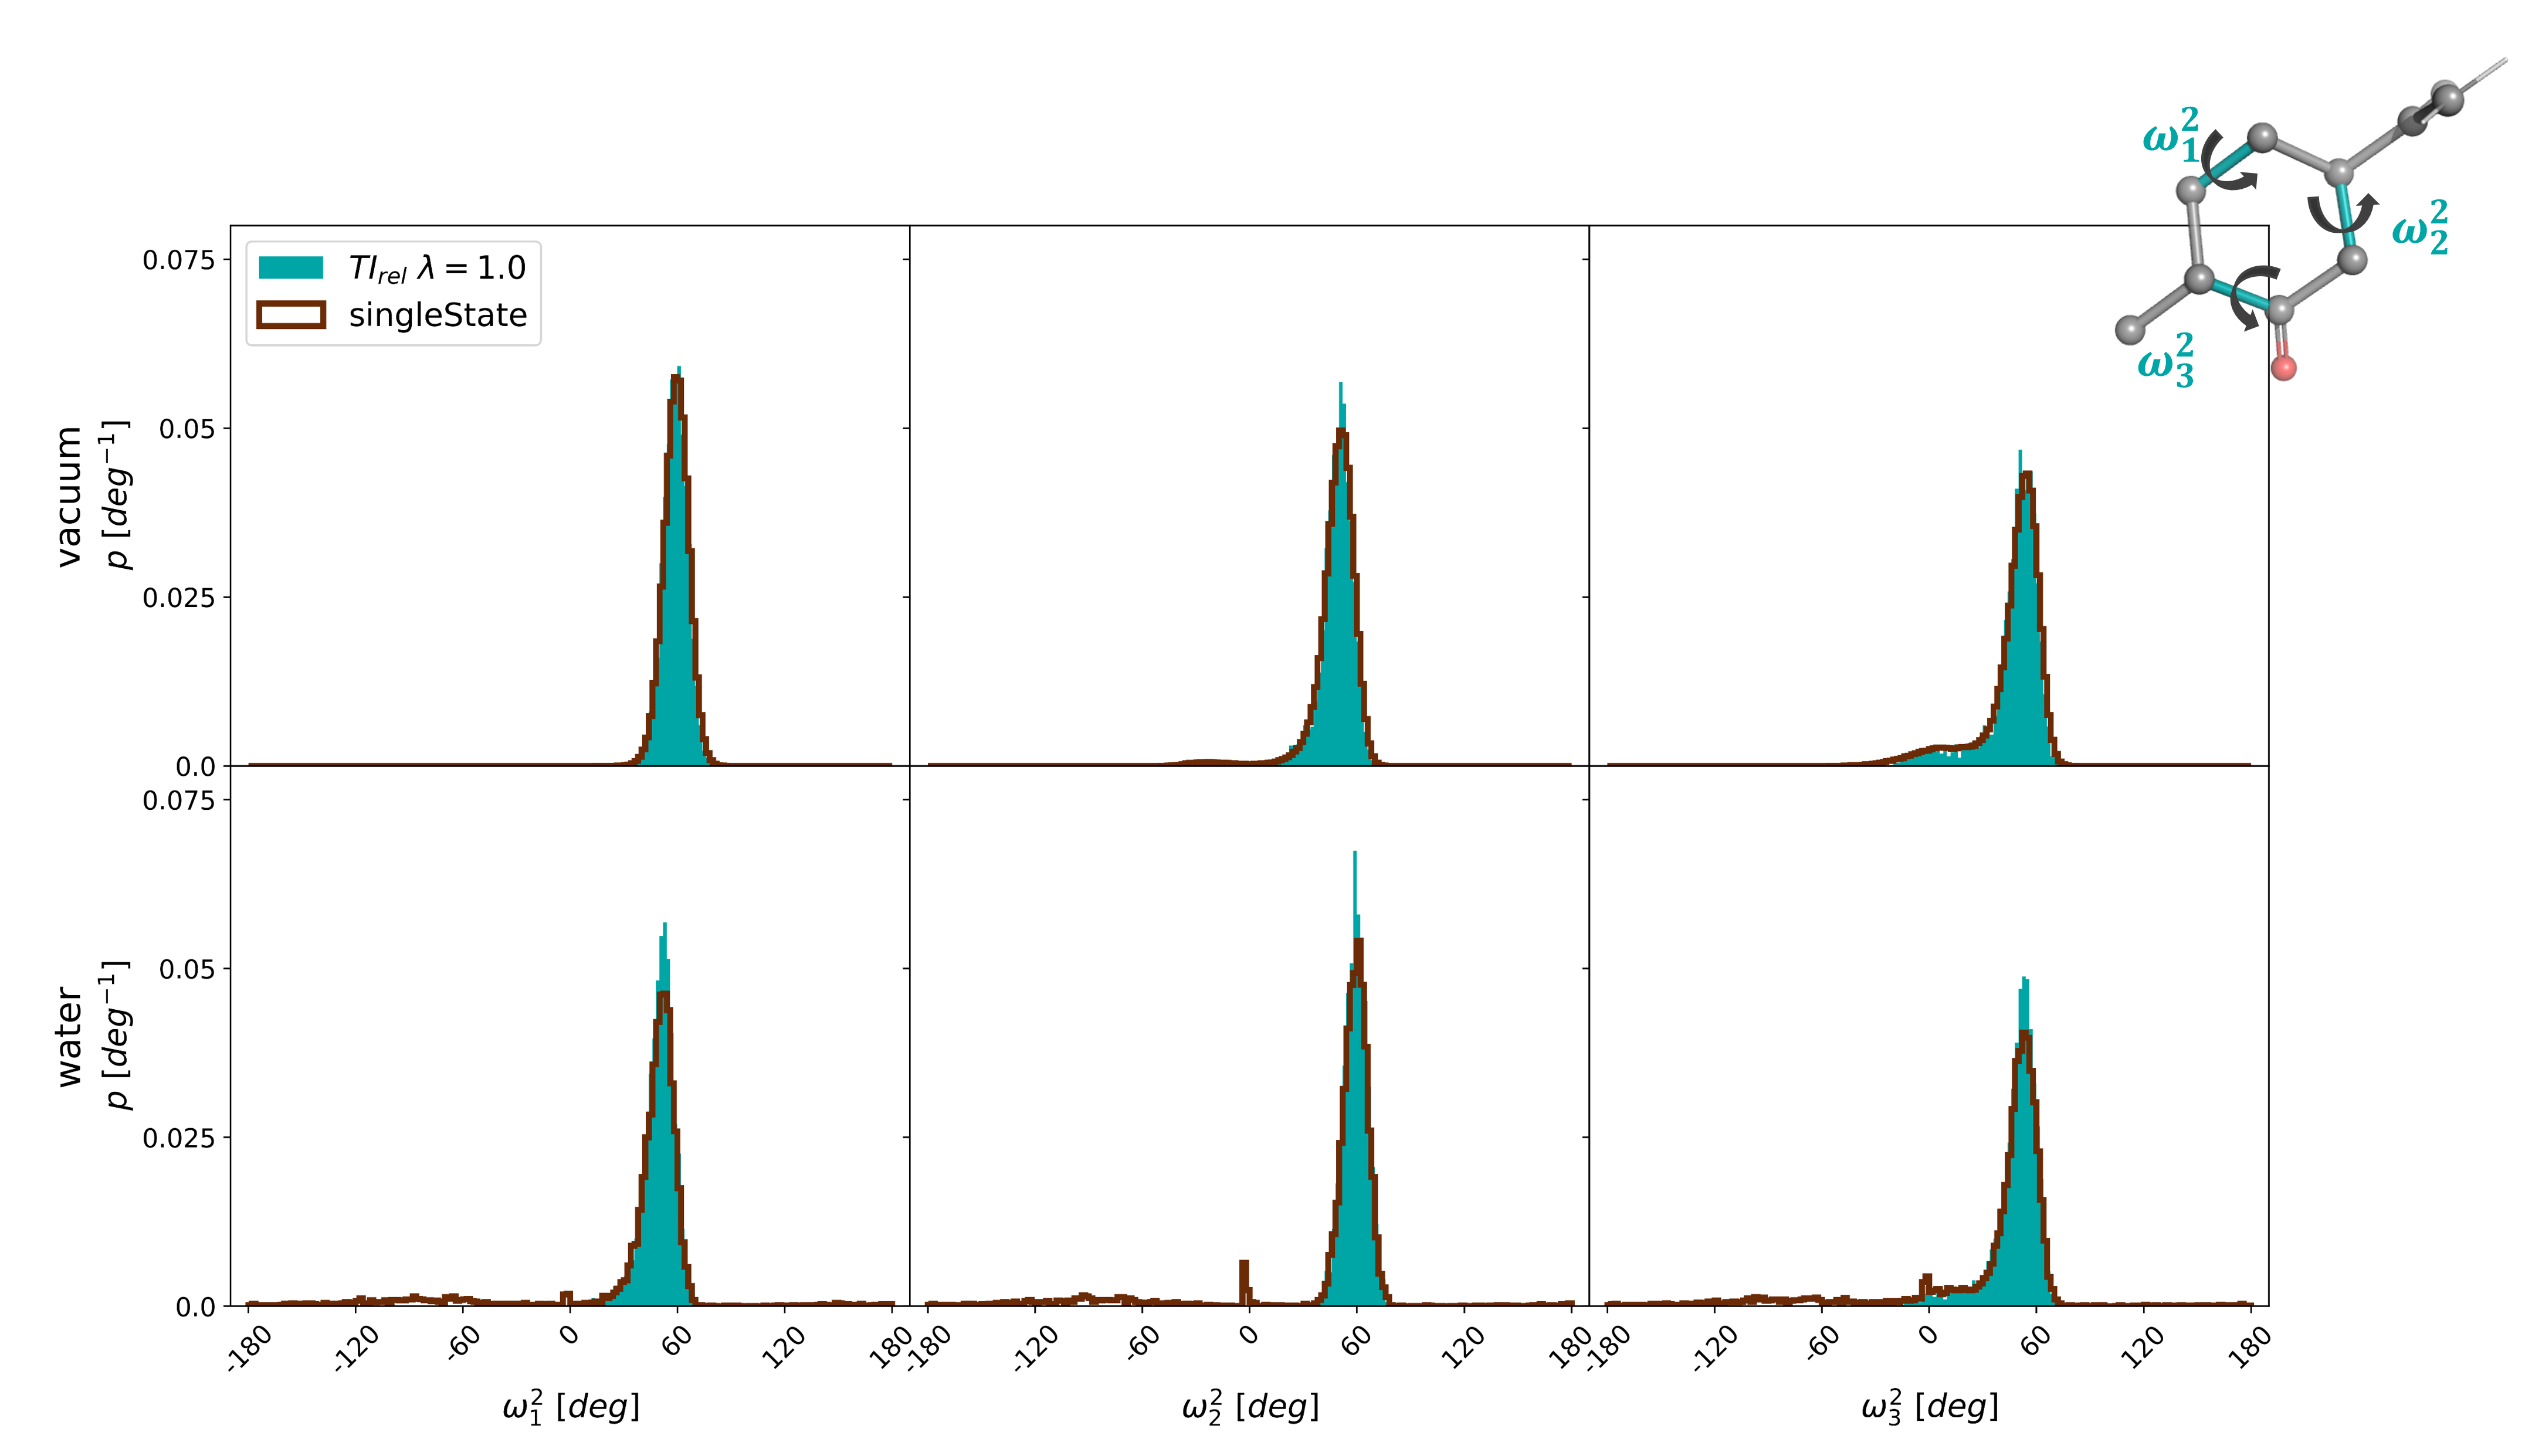
\includegraphics[width=\textwidth]{fig/results/pairwise/sampling/torsions/TI_O70_rtorsion_ana_partnerM030_singleState_populations_total.png}
        \end{subfigure}
    \begin{subfigure}{0.85\columnwidth}
        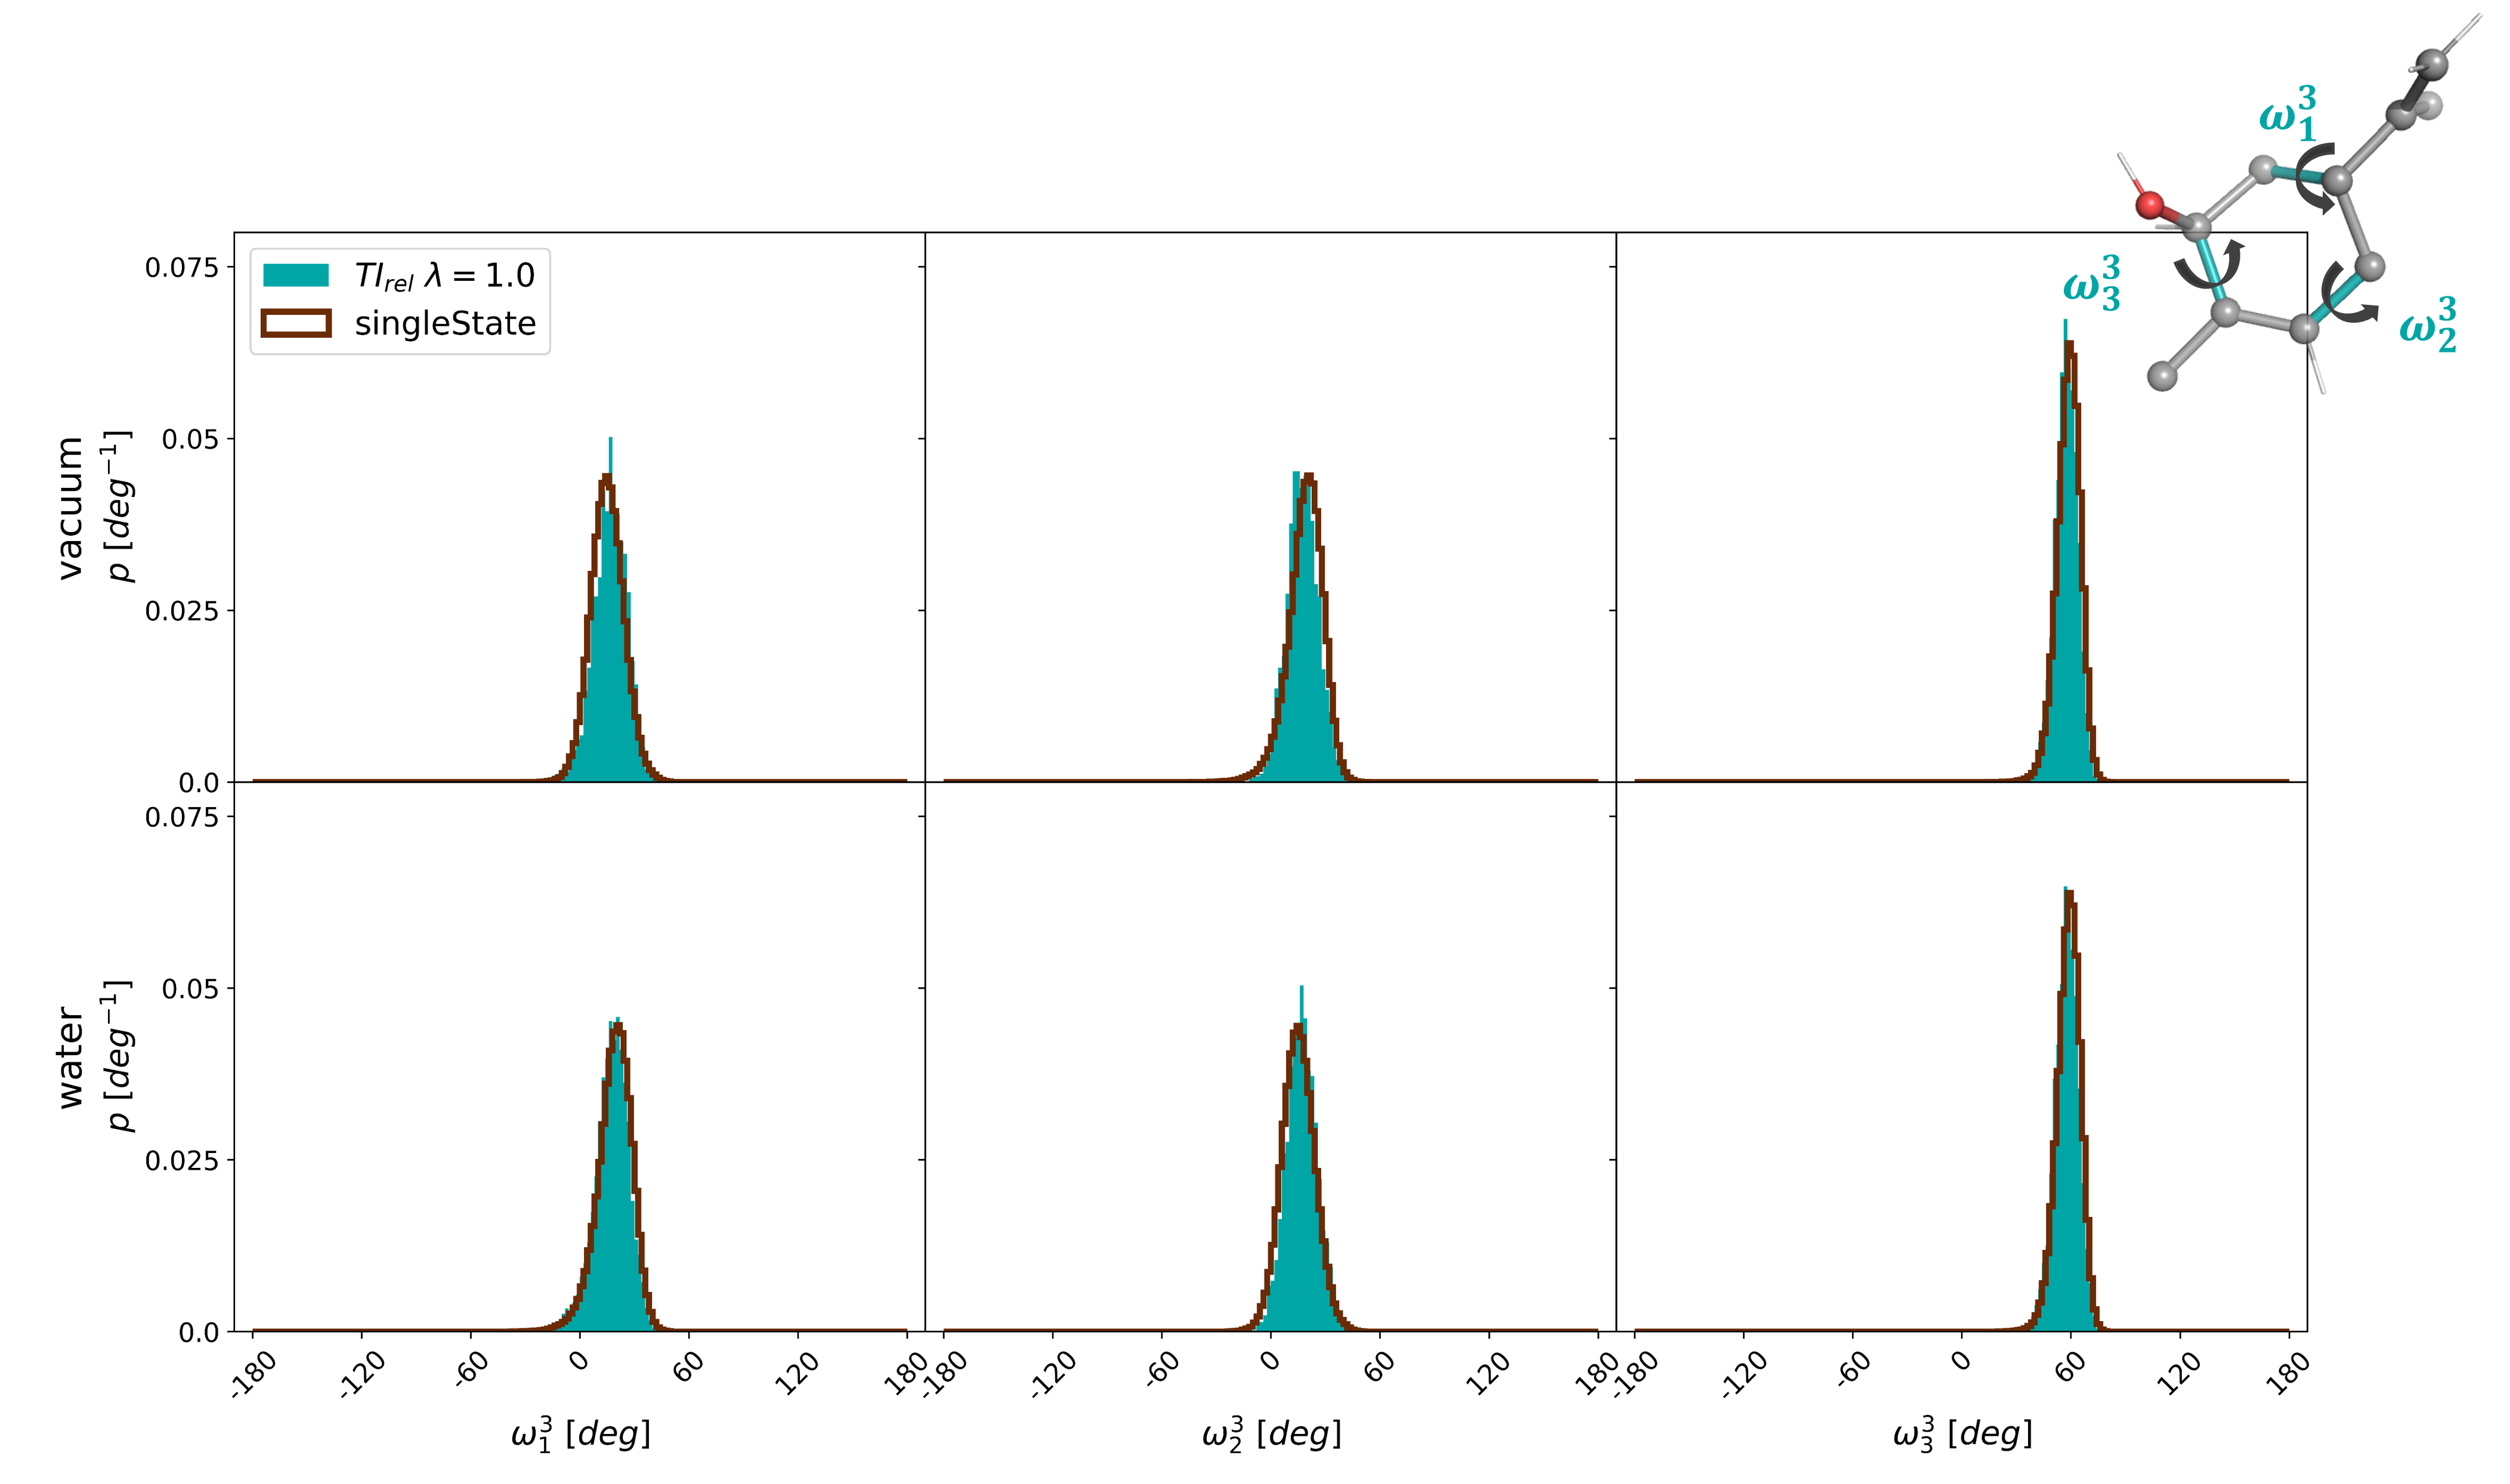
\includegraphics[width=\textwidth]{fig/results/pairwise/sampling/torsions/TI_O71_rtorsion_ana_partnerM030_singleState_populations_total.png}
        \end{subfigure}
    \caption{Comparison of the normalized torsional angle distributions of the three pseudo torsional angles of the aliphatic ring of molecules \textbf{2} (top) and \textbf{3} (bottom) in the TI calculation at $\lambda=1.0$ (filled) and in plain MD simulations (dark red line) in vacuum (top) and in water (bottom).}
    \label{fig: TIringTorisions}
\end{figure}

%Torsion analysis:
While most of the molecule pairs in Figure \ref{fig: Pairwise_TI_M030_Graph} have the same central benzene core, the transformations from molecule \textbf{12} to molecules \textbf{2} and \textbf{3} involve the change from benzene to cyclohexane or cyclohexene, respectively. To assess whether the applied distance restraints affect the conformational sampling of the aliphatic ring, the distributions of the three pseudo torsional angles (Pickett and Strauss coordinates \cite{Strauss1970}) were monitored in the simulation at $\lambda=1.0$, and compared to plain MD simulations of molecules \textbf{2} and \textbf{3} in vacuum and in water (Figure \ref{fig: TIringTorisions}).
In both cases, the distributions showed nearly perfect overlap, indicating that the sampling is not affected by the distance restraints in the linked dual topology.

\begin{figure}[h!]
    \centering
    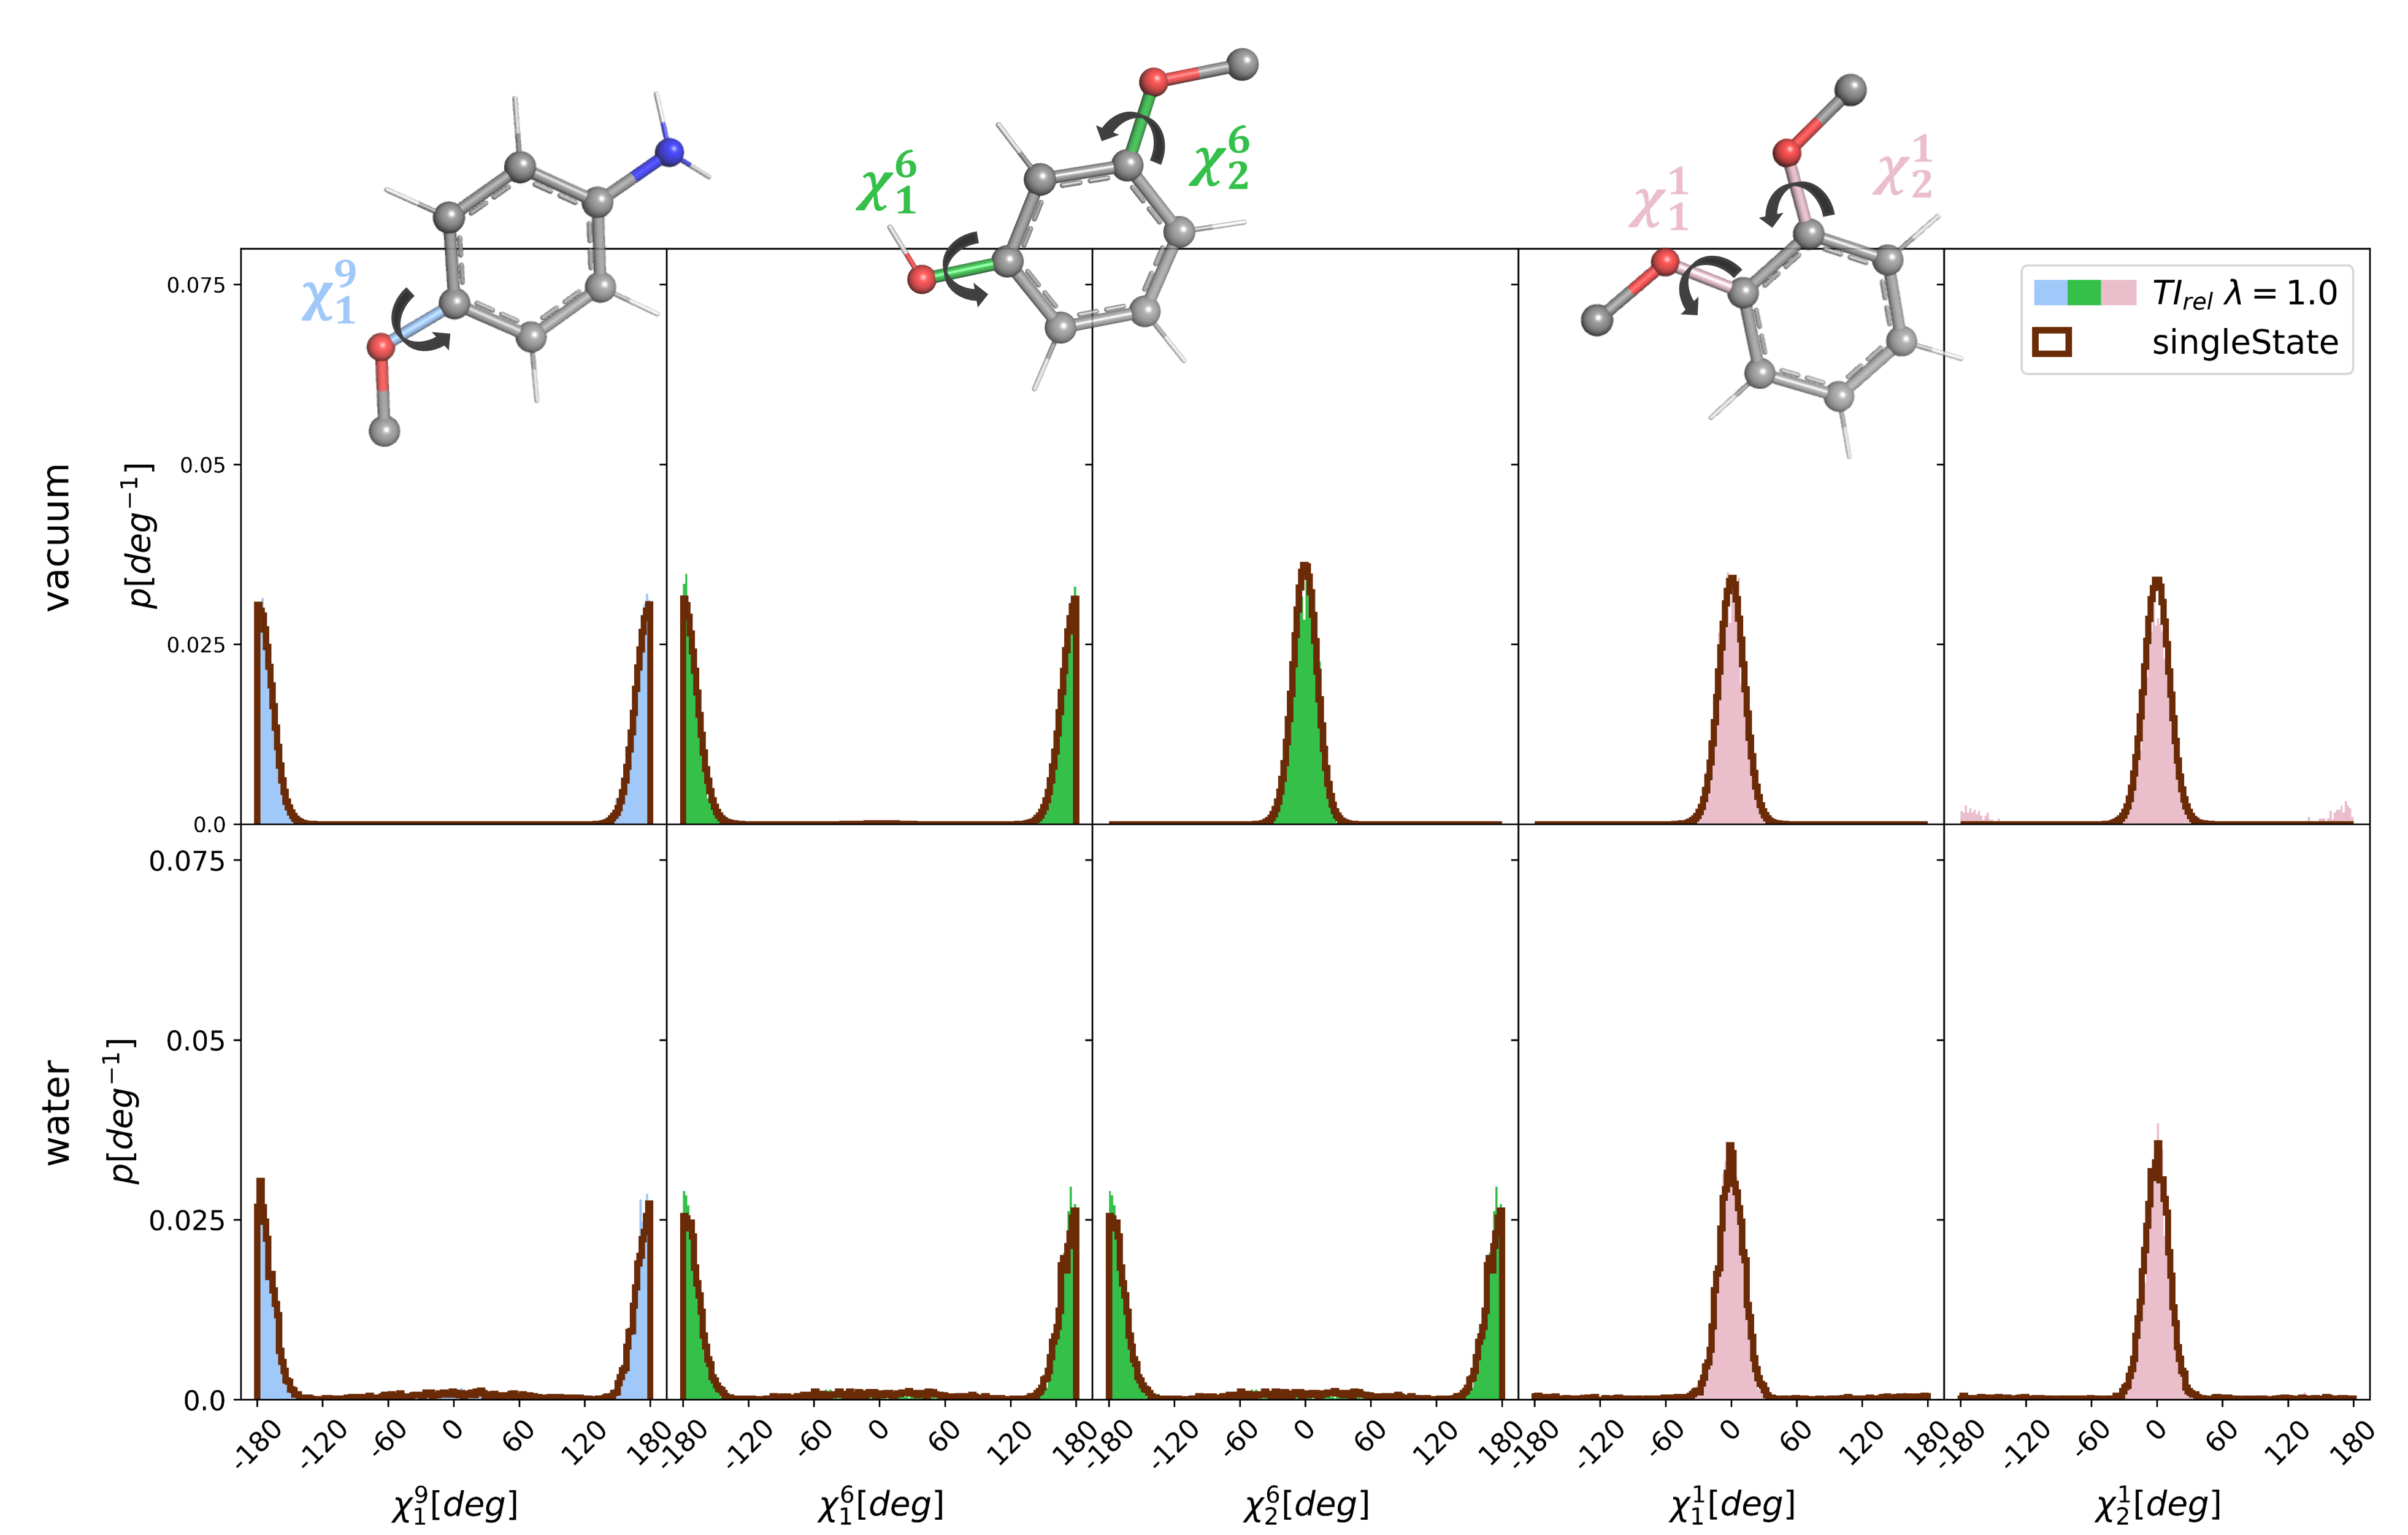
\includegraphics[width=\textwidth]{fig/results/pairwise/sampling/torsions/TI_all_substorsion_ana_partnerM030_singleState_populations_total.png}
    \caption{Comparison of the normalized torsional angle distributions of the substituents of molecules 9 (blue), 6 (green), and 1 (pink) in the simulation at $\lambda=1.0$ (filled) and in plain MD simulations (dark red line) in vacuum (top) and in water (bottom).}
    \label{SIfig: TIsubsTorisions}
\end{figure}
A similar analysis of the torsional angle distributions was also carried out for the substituents of molecules \textbf{1}, \textbf{6} and \textbf{9} (Figure \ref{SIfig: TIsubsTorisions}). Again, no major differences are observed between $\lambda=1.0$ and the plain simulations. 



